\documentclass[11pt,a4paper]{article}
\usepackage[utf8]{inputenc}
\usepackage[T1]{fontenc}
\usepackage{lmodern}
\usepackage[english]{babel}
\usepackage{amsmath}
\usepackage{amssymb}
\usepackage{amsfonts}
\DeclareMathOperator*{\argmax}{arg\,max}
\DeclareMathOperator*{\argmin}{arg\,min}
\usepackage{booktabs}
\usepackage{array}
\usepackage{multirow}
\usepackage{tabularx}
\usepackage{graphicx}
\usepackage[colorlinks=true,linkcolor=blue,citecolor=blue,urlcolor=blue]{hyperref}
\usepackage{url}
\usepackage[numbers,sort&compress]{natbib}
\usepackage[margin=2.5cm]{geometry}
\usepackage{setspace}
\onehalfspacing
\usepackage{enumitem}

\begin{document}

\title{Audio-Language Models under Psychometric Degradations: Optimization for Voice Activity Detection}
\author{Gabriel Bibbó, Mark D. Plumbley}
\date{\today}
\maketitle

\begin{abstract}
Researchers increasingly use Large Audio-Language Models (LALMs) for general audio understanding, yet we do not know how reliably they detect low-level events in degraded audio. We evaluate how LALMs perform Voice Activity Detection (VAD) and how model architecture interacts with optimization methods. We test a $3 \times 3$ experimental matrix covering three model configurations (Qwen2-Audio Base, Qwen2-Audio with LoRA, and Qwen3-Omni frozen) paired with three prompting levels: Baseline, OPRO-LLM (generative), and OPRO-Template (deterministic). We use a psychometric protocol with 22 degradation conditions spanning four acoustic axes:
segment duration, signal-to-noise ratio, reverberation, and spectral filtering. We apply strict post-selection VAD filtering to preserve label integrity during training and evaluation.

We compare two prompting paradigms, open-ended generation (OPRO-LLM) versus constrained deterministic templates (OPRO-Template), to quantify their effect on detection stability. We found a clear hierarchy of robustness: while the frozen MoE architecture (Qwen3-Omni) demonstrates superior "out-of-the-box" robustness compared to the dense baseline, parameter-efficient fine-tuning (LoRA) on the smaller dense model ultimately achieves the highest resilience to extreme noise and short durations. OPRO also recovers performance in frozen models, though the model's intrinsic temporal resolution bounds its effectiveness. By analyzing performance drop-offs, we derive task-specific "temporal integration limits" for these architectures under controlled conditions, a proxy for their minimum reliable decision window. Our results suggest that while architectural scaling improves general resistance, targeted weight adaptation remains necessary for robustness-sensitive acoustic sensing.

\noindent\textbf{Keywords:}
Large audio--language models,
robust voice activity detection,
Mixture-of-Experts,
psychometric evaluation,
Automatic Prompt Optimization (OPRO),
Low-Rank Adaptation (LoRA),
temporal resolution.
\end{abstract}

\section{Introduction}
\label{sec:introduction}

Voice Activity Detection (VAD) and Sound Event Detection (SED) enable speech recognition, diarization, and forensic analysis. While classical deep learning approaches have matured, they often fail when acoustic conditions differ from training distributions~\cite{mihalache2022using,wang2025sincqdr,bibbo2025room}. Large Audio-Language Models (LALMs) process audio through generalized instruction following, offering a new paradigm. However, we poorly understand whether these semantic capabilities translate to robust, low-level event detection under severe degradation.

\subsection{Problem Statement and Motivation}
\label{subsec:motivation}

How should one adapt a LALM that fails under acoustic degradation? Recent work has explored three representative strategies: (i)~scaling, where larger models trained on diverse acoustic conditions demonstrate improved noise robustness~\cite{radford2023whisper, hu2024large, li2025sseu}; (ii)~parameter adaptation, using Low-Rank Adaptation (LoRA) to specialize internal representations for acoustic domains~\cite{hu2022lora, yu2024investigating, wang2025lope}; or (iii)~instruction optimization, using Automatic Prompt Optimization to align behavior without weight updates~\cite{yang2023large, ramnath2025systematic}. However, no systematic comparison exists for these approaches in the context of acoustic robustness for LALMs, a gap this work addresses.

To test whether scaling alone improves robustness, we compare Qwen2-Audio~\cite{chu2024qwen2}, an open-weight dense LALM, against Qwen3-Omni (30B MoE), asking whether its mixture-of-experts architecture offers intrinsic gains under acoustic degradation. While recent work positions LALMs as high-level reasoners~\cite{ghosh2024gama}, their behavior as fine-grained detectors under varying noise, reverberation, and segment duration remains untested~\cite{li2025sseu}. Following psychoacoustic methodology (Section~\ref{subsec:psychoacoustic}), we sweep across degradation levels to build robustness curves that expose where each strategy breaks down.

\subsection{Contributions}
\label{subsec:contributions}

No prior work has tested LALMs as acoustic detectors under combined prompt optimization and acoustic stress. We make four contributions:

\begin{enumerate}
    \item \textbf{Psychometric evaluation protocol.} Standard benchmarks report accuracy at one or two SNR levels. We instead sweep 22 conditions per sample (six SNR levels, $-10$ to $+20$\,dB; four reverberation targets including dry; and durations from 20 to 1000\,ms) following the parametric approach used in human speech intelligibility studies~\cite{macpherson2014variations, kocinski2016time}.
    
    \item \textbf{Architecture--adaptation matrix.} We test three models (Qwen2-Audio base, Qwen2-Audio + LoRA, Qwen3-Omni MoE) under three prompting strategies (baseline, OPRO-LLM, OPRO-Template). This $3 \times 3$ design separates gains from scaling, fine-tuning, and prompt engineering.
    
    \item \textbf{Generative vs.\ deterministic prompt optimization.} OPRO-LLM generates natural-language instructions via a meta-LLM; OPRO-Template selects from a fixed library of structured formats. All evaluation uses open-ended generation with post-hoc normalization. We measure which optimization paradigm degrades faster under noise and how prompt structure interacts with model adaptation state.
    
    \item \textbf{Temporal integration limits.} Performance drops sharply below a threshold duration. We identify this threshold for each model, a practical bound for real-time deployment.
\end{enumerate}

\subsection{Paper Organization}
\label{subsec:organization}

Section~\ref{sec:background} reviews prior work on robust detection, psychoacoustics, and prompt optimization. Section~\ref{sec:method} details the psychometric framework, the OPRO implementation, and the LoRA training setup. Section~\ref{sec:setup} describes the experimental setup, including datasets, model configurations, and evaluation metrics. Section~\ref{sec:results} presents the experimental results and analyzes the trade-offs between architectural scale and adaptation depth.

\section{Background and Related Work}
\label{sec:background}

%%%%%%%%%%%%%%%%%%%%%%%%%%%%%%%%%%%%%%%%%%%%%%%%%%%%%%%%%%%%%%%%%%%%%%%%%%%%%%%

\subsection{Audio Detection: From Classical Systems to LALMs}
\label{subsec:audio_detection_evolution}

VAD and SED sit at the base of most audio processing pipelines. When they fail, everything downstream fails: speech recognition yields unreliable output, speaker diarization misses turns, forensic analysis becomes unusable~\cite{mihalache2022using,turpault2021sound}. Multiple studies document these failures across acoustic dimensions: detection collapses from high to 18\% F1 when SNR drops from 30~dB to $-5$~dB~\cite{papadimitriou2020audio}, degrades 15\% F-score with reverberation~\cite{turpault2021sound,bibbo2025room}, and suffers further when events overlap or frequency content changes~\cite{de2021analysis,wang2025sincqdr}.

These failures are well-documented individually, but existing benchmarks typically report aggregate metrics or focus on a single degradation type (e.g., noise), failing to isolate how distinct acoustic factors—such as reverberation vs. duration—individually impact model failure modes. Without systematic coverage across multiple axes, we cannot determine why a model fails or which degradation dominates in a given scenario.

\paragraph{Architectural evolution.}
Transformer-based models have largely supplanted convolutional and recurrent architectures for audio detection~\cite{ZAMAN2025104956}, though they still fail to generalize across acoustic domains~\cite{de2021analysis,bibbo2025room}.

Large Audio-Language Models (LALMs) represent the next paradigm shift, integrating audio encoders with pretrained LLMs to enable free-form text generation for diverse audio tasks~\cite{ghosh2024gama,wang2025u,chu2024qwen2}. GAMA~\cite{ghosh2024gama} combines a frozen LLaMA-2 backbone with multiple audio representation pathways, achieving 8--58\% improvements over baselines on reasoning benchmarks. U-SAM~\cite{wang2025u} employs specialized encoders for speech, general audio, and music, demonstrating generalization to unseen tasks.

\paragraph{Dense vs.\ Mixture-of-Experts architectures.}
Two design philosophies dominate current LALMs. Dense models activate all parameters for every input token. Mixture-of-Experts (MoE) models route each token to a subset of specialized ``experts,'' enabling large parameter counts with lower inference cost~\cite{shazeer2017outrageously}.

Qwen2-Audio~\cite{chu2024qwen2} is a dense model: a Whisper-large-v3 encoder coupled with the Qwen-7B language model, with all 7B parameters active per token. Its open weights have made it a common baseline in academic research, and its architecture supports both LoRA fine-tuning~\cite{bn2025finetuning} and prompt-level adaptation. We select Qwen2-Audio over alternatives like GAMA because its encoder--LLM integration allows LoRA to directly adapt the language model weights; GAMA freezes its LLaMA-2 backbone entirely, precluding deep parameter adaptation.

In contrast, Qwen3-Omni takes the MoE path. With 30.5B total parameters but only 3.3B activated per token, it promises the representational capacity of a much larger model at reduced compute. The hypothesis, common in recent scaling literature, is that MoE models exhibit stronger zero-shot generalization due to expert diversity~\cite{hu2024large}. We test this hypothesis under acoustic stress: can the intrinsic robustness of a frozen MoE architecture rival that of a fine-tuned dense model without requiring parameter updates?

This gap extends to LALMs. Recent work has stressed these models with adversarial attacks~\cite{hou2025evaluating} and evaluated them on question-answering benchmarks~\cite{yang2025multi,li2025sseu}, but no study has systematically tested LALMs as binary acoustic detectors under parametric degradation. Can a model that answers questions about audio also reliably detect whether speech is present in a noisy, reverberant, 50~ms clip?

%%%%%%%%%%%%%%%%%%%%%%%%%%%%%%%%%%%%%%%%%%%%%%%%%%%%%%%%%%%%%%%%%%%%%%%%%%%%%%%
\subsection{Psychoacoustic Foundations for Evaluation Design}
\label{subsec:psychoacoustic}

Human speech perception research provides empirical grounding for our choice of degradation parameters~\cite{macpherson2014variations,kocinski2016time,cueille2022effects,studebaker1987articulation}. We organize our evaluation around four axes, each targeting a distinct perceptual mechanism.

\paragraph{Signal-to-noise ratio (SNR).} MacPherson and Akeroyd~\cite{macpherson2014variations} surveyed 885 psychometric functions and found that intelligibility slopes vary from 1\% to 44\% per dB depending on masker type. Stationary noise produces the steepest slopes, as it offers no temporal gaps for signal glimpsing, making it the most demanding condition for energetic masking. We use additive white Gaussian noise across six SNR levels as a rigorous baseline.

\paragraph{Reverberation.} Cueille et al.~\cite{cueille2022effects} showed that reverberation degrades intelligibility through temporal smearing, a mechanism distinct from the energetic masking caused by additive noise. Late reflections blur phonetic boundaries and reduce temporal modulation depth. To isolate this factor's contribution to LALM failure, we vary reverberation time (RT60) independently from other degradations.

\paragraph{Spectral filtering.} The Speech Intelligibility Index~\cite{studebaker1987articulation} quantifies how different frequency bands contribute to comprehension, with the 1--4~kHz range carrying the highest weight for consonant recognition. Bandwidth limitations (from telephone-quality narrowband to wideband transmission) alter the spectral cues available for detection. We apply bandpass filtering to test whether LALMs rely on specific frequency regions or exhibit robustness across spectral configurations.

\paragraph{Segment duration.} Human temporal integration for speech recognition has a lower bound around 75--100~ms; below this threshold, performance collapses~\cite{kocinski2016time}. We sweep segment duration from 20~ms to 1000~ms to locate analogous integration limits in LALMs. The shortest duration at which a model maintains reliable detection serves as an empirical measure of its temporal resolution, a practical bound for real-time deployment.

%%%%%%%%%%%%%%%%%%%%%%%%%%%%%%%%%%%%%%%%%%%%%%%%%%%%%%%%%%%%%%%%%%%%%%%%%%%%%%%
\subsection{Temporal Limitations of LALMs}
\label{subsec:temporal_limitations}

Audio Question Answering (AQA) has emerged as a benchmark for acoustic reasoning~\cite{yang2025multi,dcase2025task5aqa}. Baseline evaluations exposed large gaps: Qwen2-Audio achieved only 30--52\% accuracy across subsets, with qualitative analysis revealing hallucinations, timestamp imprecision, and confusion between perceptually similar sounds. AQA and our VAD evaluation share the same underlying models but differ in abstraction: AQA poses multiple-choice questions requiring inference, while we apply LALMs to binary classification of voice presence, a simpler semantic decision that exposes low-level robustness rather than high-level reasoning.

LALMs struggle with fine-grained temporal processing~\cite{wang2025timeaudio,sridhar-etal-2025-enhancing}. Wang et al.~\cite{wang2025timeaudio} traced these ``temporal gaps'' to architectural choices: temporal downsampling in projection layers destroys the resolution needed for accurate timestamp localization. Their TimeAudio framework introduces explicit temporal markers and time-aware encoding, improving performance on temporal grounding tasks.

Sridhar et al.~\cite{sridhar-etal-2025-enhancing} found that LALMs achieve only 22\% accuracy on temporal reasoning benchmarks for AQA. Targeted data augmentation and curriculum learning helped, but without careful training strategies models ``overfit to temporal reasoning'' while ``forgetting base capabilities.'' In classical SED, Ren et al.~\cite{ren2025group} identified a related conflict: event classification requires global representations, while temporal localization depends on high-resolution local features.

These findings confirm that LALMs are not naturally fine-grained temporal processors, reinforcing our decision to evaluate clip-level VAD before attempting temporal grounding.

%%%%%%%%%%%%%%%%%%%%%%%%%%%%%%%%%%%%%%%%%%%%%%%%%%%%%%%%%%%%%%%%%%%%%%%%%%%%%%%
\subsection{Adaptation Strategies: Input Space vs.\ Parameter Space}
\label{subsec:adaptation}

When a LALM fails on a target task, two adaptation paths exist. \textit{Input-space adaptation} modifies prompts while keeping model weights frozen; this includes manual prompt engineering and automatic prompt optimization. \textit{Parameter-space adaptation} modifies the model itself, with Low-Rank Adaptation (LoRA) as the dominant efficient method~\cite{hu2022lora}.

These strategies differ in cost, data requirements, and failure modes. Prompt optimization requires no training data beyond a small validation set, but operates within the model's existing capabilities. LoRA requires labeled examples and compute, but can shift the model's internal representations toward the target domain. Recent work suggests LoRA is particularly effective for acoustic domain adaptation~\cite{yu2024investigating,wang2025lope,bn2025finetuning}, though systematic comparisons under degradation are scarce.

Our experimental design tests both paths. We apply OPRO~\cite{yang2023large} to optimize prompts for Qwen2-Audio (input-space), and LoRA to fine-tune Qwen2-Audio on curated, high-quality VAD data (parameter-space). Qwen3-Omni serves as a frozen baseline, testing whether architectural scaling alone, without any adaptation, suffices for robustness.

\subsubsection{Prompt Optimization and the Decoding Constraint Debate}
\label{subsubsec:apo}

Hou et al.~\cite{hou2025evaluating} evaluated LALM robustness against audio injection attacks
and found that no model demonstrated consistent resistance. A negative correlation emerged
between instruction-following capability and injection robustness, suggesting that the
audio-text input channel is inherently sensitive to perturbations. We extend this concern
from adversarial to acoustic perturbations, hypothesizing that natural degradations (noise,
reverberation, short duration) may similarly destabilize model behavior.

Automatic Prompt Optimization treats prompt design as a search problem: find the instruction that maximizes performance on a validation set~\cite{ramnath2025systematic,CHEN2025101260}. OPRO~\cite{yang2023large} implements this by having the LLM itself propose and refine prompt candidates. Zhang et al.~\cite{zhang2024revisiting} showed this works best with capable base models.

A related but distinct question is whether constraining the model's output space can
mitigate this instability. \textit{Constrained decoding} restricts outputs to a small token set
(e.g., ``A'' or ``B''), eliminating parsing ambiguity but potentially discarding useful
acoustic reasoning. \textit{Open decoding} allows free-form generation, permitting richer responses
but introducing extraction noise under acoustic stress. The trade-off between these paradigms
for audio tasks is unclear; we test both strategies and compare their robustness curves
in Section~\ref{sec:results}.

\subsubsection{Parameter-Efficient Fine-Tuning with LoRA}
\label{subsubsec:lora}

Low-Rank Adaptation (LoRA)~\cite{hu2022lora} inserts trainable low-rank matrices into frozen pretrained weights. For a weight matrix $W \in \mathbb{R}^{d \times k}$, LoRA learns $\Delta W = BA$ where $B \in \mathbb{R}^{d \times r}$ and $A \in \mathbb{R}^{r \times k}$, with rank $r \ll \min(d,k)$. This reduces trainable parameters by orders of magnitude while preserving the pretrained model's general capabilities.

Recent work demonstrates LoRA's effectiveness for acoustic adaptation. Yu et al.~\cite{yu2024investigating} found that LoRA fine-tuning improves speech recognition robustness, though advanced variants like dynamic rank allocation can reduce adversarial robustness. Wang et al.~\cite{wang2025lope} proposed LoPE, which uses asymmetric LoRA experts specifically for noise robustness. For LALMs, BN et al.~\cite{bn2025finetuning} fine-tuned Qwen2-Audio with LoRA for temporal localization in therapy sessions, achieving clinically useful precision.

These results suggest LoRA can specialize LALMs for challenging acoustic conditions. We fine-tune Qwen2-Audio with LoRA on clean, VAD-filtered speech segments, then evaluate under unseen degradations. Unlike data augmentation approaches that train on noisy examples, we test whether adaptation on clean data alone improves robustness. LoRA training also teaches the model to respond in a strict binary format, reducing reliance on post-hoc normalization. This sets up a direct comparison: can prompt optimization alone match the gains from parameter adaptation?

%%%%%%%%%%%%%%%%%%%%%%%%%%%%%%%%%%%%%%%%%%%%%%%%%%%%%%%%%%%%%%%%%%%%%%%%%%%%%%%
 %V2

%%%%%%%%%%%%%%%%%%%%%%%%%%%%%%%%%%%%%%%%%%%%%%%%%%%%%%%%%%%%%%%%%%%%%%%%%%%%%%%
\section{Proposed Methodology}
\label{sec:method}
%%%%%%%%%%%%%%%%%%%%%%%%%%%%%%%%%%%%%%%%%%%%%%%%%%%%%%%%%%%%%%%%%%%%%%%%%%%%%%%

\subsection{Overview of the Framework}
\label{subsec:overview}

We evaluate and adapt Large Audio--Language Models (LALMs) for clip-level Voice Activity Detection (VAD) under controlled psychometric degradations. The pipeline proceeds as follows: (i)~extract base clips of 1000\,ms from source datasets, each labeled as SPEECH or NONSPEECH; (ii)~apply a bank of 22 psychometric degradation conditions spanning segment duration, signal-to-noise ratio (SNR), reverberation, and spectral filtering; (iii)~embed each degraded segment in a fixed 2000\,ms container padded with low-amplitude Gaussian noise, keeping the informative region centered; (iv)~query the target LALM with a VAD prompt asking whether the clip contains human speech; and (v)~normalize the model's textual response to a SPEECH/NONSPEECH label for metric computation.

This evaluation adopts a psychometric-style approach, treating accuracy as a function of each degradation parameter. By sweeping duration from 20 to 1000\,ms while fixing other factors at neutral values, we trace accuracy-versus-duration curves analogous to classical temporal integration functions. Similarly, varying SNR from $-10$ to $+20$\,dB yields noise robustness curves. To disentangle the effects of architecture, parameter adaptation, and prompting, we employ a symmetric $3 \times 3$ experimental matrix crossing \textit{Model Configuration} with \textit{Prompting Strategy}. The three model configurations are: (i)~Qwen2-Audio (Base); (ii)~Qwen2-Audio with Low-Rank Adaptation (LoRA); and (iii)~Qwen3-Omni evaluated as a frozen Mixture-of-Experts (MoE) model. The three prompting strategies are: (i)~a hand-crafted baseline prompt; (ii)~OPRO-LLM, a generative prompt optimizer that searches in free-text instruction space; and (iii)~OPRO-Template, a deterministic optimizer that searches over a fixed library of structured templates. All nine cells are evaluated on the same psychometric bank (Section~\ref{sec:results}).

\paragraph{Preliminary tuning and input conditioning.} Prior to the systematic evaluation, we conducted a pilot study to establish a competitive baseline configuration. Qwen2-Audio exhibited performance instability when processing raw clips shorter than 1000\,ms, likely due to distribution shifts from its pre-training data. To mitigate this without introducing pitch artifacts from time-stretching, we standardized the input format as described in Section~\ref{subsec:degradation_bank}. Similarly, the baseline prompt was selected through manual iterative testing to verify that it effectively primes the model for binary classification, establishing a solid reference point against which the automated optimization methods are compared.

\subsection{Psychometric Degradation Bank}
\label{subsec:degradation_bank}

The degradation bank transforms each base clip into 22 variants along four independent dimensions, as summarized in Table~\ref{tab:degradation_bank}. When varying one dimension, the others are fixed at neutral values: 1000\,ms duration, no added noise, no reverberation (T60 $= 0$), and no spectral filtering. All variants are embedded in a 2000\,ms container with symmetric padding using Gaussian noise of amplitude $\sigma = 10^{-4}$. This low-amplitude padding serves two purposes: it avoids numerical issues (e.g., division-by-zero or ill-defined SNR values) in subsequent processing stages, and it stabilizes the model's encoder by providing an input length consistent with its effective attention window (see Section~\ref{subsec:overview}). The padding signal lies well below any plausible detection threshold and does not carry discriminative information; no time-stretching or content-aware augmentation is applied.

\begin{table}[t]
\centering
\caption{Summary of the psychometric degradation bank (22 variants per base clip).}
\label{tab:degradation_bank}
\footnotesize
\setlength{\tabcolsep}{3pt}
\renewcommand{\arraystretch}{1.15}

\begingroup
\sloppy
\begin{tabular}{p{0.18\linewidth} p{0.28\linewidth} p{0.46\linewidth}}
\hline
\textbf{Axis} & \textbf{Condition} & \textbf{Values} \\
\hline
Segment duration &
Centered segment length &
20, 40, 60, 80, 100, 200, 500, 1000\,ms (8) \\
\hline
SNR &
Added white-noise SNR &
$-10$, $-5$, 0, $+5$, $+10$, $+20$\,dB (6) \\
\hline
Reverberation (T60) &
Target T60 (RIR convolution) &
0.0, 0.3, 1.0, 2.5\,s (4); for non-zero targets, select RIRs within $\pm 0.2$\,s \\
\hline
Spectral filtering &
Butterworth filter type &
None; bandpass 300--3400\,Hz; lowpass 3400\,Hz; highpass 300\,Hz (4) \\
\hline
\end{tabular}

\vspace{0.5ex}
\parbox{\linewidth}{\footnotesize\textit{Note:} When varying one axis, all other axes are held at their neutral settings (see text). Each variant is padded symmetrically with Gaussian noise ($\sigma=10^{-4}$) to a 2000\,ms container.}
\endgroup
\end{table}

\subsubsection{Segment Duration Conditions}
\label{subsubsec:duration}

We extract centered segments of 20, 40, 60, 80, 100, 200, 500, and 1000\,ms from each base clip, yielding eight duration conditions. The grid from 20 to 1000\,ms spans from sub-frame windows at or below the encoder's effective frame rate ($\approx$40\,ms for Whisper-style architectures) up to segments that comfortably contain several phonemes or short words. This range probes the crossover from ``too brief to decide'' to ``sufficient context for stable speech/non-speech decisions.''

If the source clip is shorter than the target duration, no time-stretching is applied: the full clip is kept and later padded to the 2000\,ms container, rather than being artificially lengthened. Shorter durations probe the model's temporal integration limit, defined as the minimum segment length at which reliable detection remains possible.

\subsubsection{SNR Manipulations}
\label{subsubsec:snr}

We add white Gaussian noise at six SNR levels: $-10$, $-5$, 0, $+5$, $+10$, and $+20$\,dB. This range covers challenging surveillance-like conditions where speech is heavily masked ($-10$ to 0\,dB), up to relatively clean conditions ($+20$\,dB), in line with prior work examining cross-SNR generalization in audio event detection~\cite{turpault2021sound}.

Noise amplitude is calibrated to the signal's Root Mean Square (RMS):
\begin{equation}
\sigma_{\text{noise}} = \frac{\text{RMS}_{\text{signal}}}{10^{\text{SNR}/20}}.
\end{equation}
The resulting mixture is clipped to $[-1, 1]$ to prevent saturation. For near-silent segments where the RMS of the effective speech/non-speech region falls below $10^{-8}$, we cannot meaningfully enforce a target SNR. In these rare cases, we add a minimal amount of Gaussian noise (RMS $= 10^{-4}$), mark the SNR as undefined, and retain the sample as an extreme low-SNR condition.

We set the fallback noise RMS to match the container padding amplitude ($\sigma = 10^{-4}$),
ensuring that near-silent segments blend seamlessly into the noise floor of the container
and cannot be distinguished from the padding region by spectral characteristics alone.

\subsubsection{Reverberation Simulation}
\label{subsubsec:reverb}

We simulate room acoustics using real Room Impulse Responses (RIRs) from the RIRS\_NOISES dataset~\cite{ko2017study}. Four reverberation conditions are defined by target T60: 0.0\,s (dry, no convolution), 0.3\,s (typical of small offices or meeting rooms), 1.0\,s (larger conference rooms), and 2.5\,s (highly reverberant spaces such as halls or atriums). For each non-zero T60, we select RIRs whose estimated reverberation time falls within $\pm 0.2$\,s of the target.

Convolution is performed via FFT, and the output is truncated to the original segment length. For very short windows (e.g., 20\,ms), this means we capture only the early part of the decay rather than the full T60 tail, but the temporal smearing of onsets is still sufficient to perturb transient cues. The resulting signal is normalized to match the original RMS before padding.

\subsubsection{Spectral Filtering}
\label{subsubsec:filtering}

We apply four spectral conditions using fourth-order Butterworth filters with zero-phase filtering: none (unfiltered), bandpass (300--3400\,Hz), lowpass (cutoff 3400\,Hz), and highpass (cutoff 300\,Hz). The 300--3400\,Hz bandpass emulates a telephone-style channel (ITU-T recommendations) that retains most of the speech energy, while the highpass (300\,Hz) and lowpass (3400\,Hz) conditions selectively remove low-frequency voicing and high-frequency consonant cues, respectively, to test how strongly the model relies on these spectral regions.

\subsection{Prompting and Output Normalization}
\label{subsec:prompting}

All evaluation conditions are formulated as instruction-following VAD. Prompts request a categorical decision and, unless stated otherwise, instruct the model to answer with exactly one of two labels (\texttt{SPEECH} or \texttt{NONSPEECH}). All inference uses greedy decoding (temperature $= 0$) for deterministic, reproducible outputs across experimental cells. While the prompting strategy changes across experimental cells (baseline vs.\ optimized prompts), the downstream evaluation requires a consistent binary label for metric computation. We therefore apply a deterministic normalization function that maps formatting variations to the canonical labels through a six-level priority hierarchy:
\begin{enumerate}[leftmargin=*]
    \item \textbf{NONSPEECH substring detection.} Case-insensitive substring match for \texttt{NONSPEECH}, \texttt{NON-SPEECH}, \texttt{NON SPEECH}, or \texttt{NO SPEECH}. This level is checked \emph{before} SPEECH to avoid false matches, since the string ``NONSPEECH'' contains ``SPEECH'' as a substring.
    \item \textbf{SPEECH substring detection.} Substring match for \texttt{SPEECH}, applied only if level~1 did not match.
    \item \textbf{Letter mapping.} When the prompt uses an A/B/C/D structure, a leading letter is mapped to the corresponding label via a prompt-specific dictionary.
    \item \textbf{YES/NO detection.} Word-boundary matching for affirmative tokens (\texttt{YES}, \texttt{TRUE}, \texttt{SI}) mapped to SPEECH, and negative tokens (\texttt{NO}, \texttt{FALSE}, \texttt{NEGATIVE}) mapped to NONSPEECH.
    \item \textbf{Keyword-based matching.} Counts of speech-related terms (e.g., \textit{voice}, \textit{talking}, \textit{spoken}; 18~terms) versus non-speech terms (e.g., \textit{noise}, \textit{silence}, \textit{music}; 29~terms), returning the dominant category when the speech count exceeds the non-speech count or vice versa.
    \item \textbf{Unknown.} If no rule matches, the response is forwarded to a heuristic fallback that scores speech indicators against non-speech indicators; if this also fails, the response is marked as invalid.
\end{enumerate}

In practice, for the OPRO-optimized prompts used in our final evaluation, all of which explicitly request \texttt{SPEECH} or \texttt{NONSPEECH} output, over 99.7\% of responses are resolved at levels~1--2 (direct substring match) for eight of the nine configurations, with Qwen3-Omni achieving 100\% parseability across all three prompting conditions. The exception is Base+OPRO-LLM, where 320 of 21{,}340 responses (1.5\%) could not be resolved to a binary label by any normalization level and were treated as invalid predictions. Qualitative inspection of these responses revealed that the majority consisted of outputs in Chinese characters, suggesting that the generative OPRO-LLM prompt occasionally triggered language-switching behavior in the base model under acoustic degradation. Levels~3--6 are primarily relevant for alternative prompt formats (A/B multiple-choice, open-ended) not used in the reported results.

Table~\ref{tab:normalization_levels} reports the normalization-level breakdown for three representative configurations re-evaluated with detailed logging. The overwhelming majority of responses fall into levels~1--2 (direct substring match), confirming that the optimized prompts successfully elicit well-formed binary outputs.

\begin{table}[t]
\centering
\caption{Normalization-level breakdown for three representative configurations on the full test set ($n = 21{,}340$). L1 = NONSPEECH substring, L2 = SPEECH substring, L5 = semantic keywords, L6b = unknown/unparseable.}
\label{tab:normalization_levels}
\footnotesize
\setlength{\tabcolsep}{4pt}
\renewcommand{\arraystretch}{1.12}
\begin{tabular}{lrrrr}
\toprule
\textbf{Configuration} & \textbf{L1 (\%)} & \textbf{L2 (\%)} & \textbf{L5 (\%)} & \textbf{L6b (\%)} \\
\midrule
Base+OPRO-LLM   & 56.56 & 41.94 & 0.00 & 1.50 \\
LoRA+OPRO-Tmpl   & 50.47 & 49.53 & 0.00 & 0.00 \\
Qwen3+Hand       & 53.66 & 46.34 & 0.00 & 0.00 \\
\bottomrule
\end{tabular}
\end{table}

\subsection{Optimization Strategies}
\label{subsec:optimization}

We consider two complementary approaches to improve LALM robustness for VAD: \textit{input-space optimization} via Automatic Prompt Optimization (OPRO), and \textit{parameter-space adaptation} via LoRA. The winning prompts produced by each optimization method are reported in Table~\ref{tab:winning_prompts}.

\subsubsection{Automatic Prompt Optimization (OPRO-LLM)}
\label{subsubsec:opro_llm}

OPRO-LLM implements a generative prompt optimizer following the Optimization by Prompting paradigm~\cite{yang2023large}. A meta-LLM (Qwen2.5-7B-Instruct, temperature $= 0.7$, top\_p $= 0.9$, max\_new\_tokens $= 2000$) iteratively proposes and evaluates candidate prompts based on evaluation feedback. The search runs for 30 iterations. In each iteration, the meta-LLM generates 3 candidate prompts, which are evaluated on the full 660-sample development set. The top-$k$ memory retains the $k=10$ highest-scoring prompts across history. Early stopping is triggered after 5 iterations without improvement. The optimization loop proceeds as follows:

\begin{enumerate}[leftmargin=*]
\item Initialize from a hand-crafted prompt and evaluate it on a fixed, class-balanced development set of 660 samples with equal representation of SPEECH and NONSPEECH under the full psychometric bank.

\item Construct a meta-prompt describing the task, the reward function, and the top-$k$ prompts with their scores. At each iteration, pass this meta-prompt to the meta-LLM, which proposes new candidate prompts.

\item The meta-LLM is instructed to generate prompts that are concise and emphasize robustness to short and noisy clips. The meta-prompt encourages diverse prompt formats (direct questions, binary choice, commands, open-ended queries).

\item Candidate prompts are sanitized by removing forbidden special tokens and enforcing a character length range, without imposing keyword restrictions. This allows OPRO-LLM to explore diverse phrasings and prompt formats freely.

\item Evaluate each candidate on the development set and compute the reward:
\begin{equation}
R = \mathrm{BA}_{\text{clip}} + \lambda \, \mathrm{BA}_{\text{cond}}, \quad \lambda = 0.25,
\end{equation}
where $\mathrm{BA}_{\text{clip}} \in [0,1]$ is the balanced accuracy computed globally over all development samples and conditions, and $\mathrm{BA}_{\text{cond}} \in [0,1]$ is the mean of balanced accuracies computed separately for each degradation axis (duration, SNR, filtering, reverberation). The resulting reward $R \in [0, 1.25]$ is used purely for ranking candidate prompts; absolute reward values are not interpretable outside this comparative context. This formulation encourages prompts that perform well across the full degradation bank rather than excelling only under clean conditions.
We set $\lambda = 0.25$ heuristically to give modest weight to per-axis uniformity without
dominating the global signal; this value was fixed throughout all experiments and was not
itself optimized. We acknowledge this as a design choice that could influence which prompts
are selected, though the final evaluation on the complete test set (21{,}340 samples) provides
the definitive performance comparison independently of the reward function used during
optimization.

\item Update the top-$k$ memory, retaining the highest-scoring prompts.

\item Repeat for a fixed number of iterations or until no improvement for several consecutive iterations (early stopping).
\end{enumerate}

This procedure represents an open-ended search in semantic space: the meta-LLM can propose any natural-language instruction, and performance is evaluated over the complete development set at each iteration. In practice, all three runs triggered early stopping well before the 30-iteration budget: Qwen2-Base converged in 10 iterations (best prompt at iteration~4), Qwen2-LoRA in 9 (best at iteration~3), and Qwen3-Omni in 8 (best at iteration~2). The decreasing exploration required by stronger models is consistent with the OPRO saturation effect discussed in Section~\ref{subsec:disc_opro_saturation}. The computational cost of OPRO-LLM is high: each iteration evaluates 3 candidates on 660 samples, yielding approximately 17{,}820 forward passes for Qwen2-Base (10 iterations), 15{,}840 for Qwen2-LoRA (9 iterations), and 14{,}520 for Qwen3-Omni (8 iterations), excluding the meta-LLM overhead.

\subsubsection{Deterministic Template Search (OPRO-Template)}
\label{subsubsec:opro_template}

While OPRO-LLM uses a meta-LLM to \textit{generate} candidate prompts, OPRO-Template replaces this generation step with \textit{selection} from a fixed library of 15 hand-designed prompt templates. The target model still produces its responses via standard generation; only the prompt proposal mechanism changes. All 15~templates request output in \texttt{SPEECH}/\texttt{NONSPEECH} label format and include variants such as strict single-token directives, contrastive definitions, one-shot examples, and conservative/liberal bias framings.

The search proceeds over $I = 15$ iterations with a budget of $K = 8$ candidate templates per iteration, evaluated on a class-balanced mini-dev set of $N = 20$ clips (stratified 50/50 SPEECH/NONSPEECH, resampled each iteration using \texttt{seed + iteration}). In the first iteration, the first $K$~templates from the library are evaluated. In subsequent iterations, the current best template is retained and the remaining $K - 1$ slots are filled by random sampling (with shuffle) from the unused portion of the library. Each candidate is scored by classification accuracy on the mini-dev subset; because the subset is class-balanced, this approximates balanced accuracy. The highest-scoring template is carried forward as the current best.

Unlike OPRO-LLM, this procedure does not compute the composite per-axis reward (Equation~2); selection is based solely on mini-dev accuracy. The small per-iteration evaluation budget ($N = 20$) makes the method computationally lightweight (requiring at most $I \times K \times N = 15 \times 8 \times 20 = 2{,}400$ forward passes per model, an order of magnitude fewer than OPRO-LLM) but introduces sampling variance across runs: with a resolution of $1/20 = 0.05$ per step, multiple templates can tie at ceiling accuracy. In our experiments, up to four templates achieved perfect scores (20/20) on different iterations for the LoRA-adapted model, indicating that the selection among top-performing templates is sensitive to the seed-determined sample sequence. Although the template library is fixed, the procedure includes controlled randomness in both template ordering and mini-dev sampling, and is fully reproducible by fixing the random seed. All results reported use seed~42; the final evaluation on the full test set (21{,}340 samples) provides the definitive performance comparison. Winning templates for each model configuration are reported in Section~\ref{sec:results}.

OPRO optimizes the prompt \textit{content}, not the decoding strategy. All nine cells in the final evaluation use open-ended generation (\texttt{max\_new\_tokens=128}) with post-hoc normalization (Section~\ref{subsec:prompting}). The framework supports a constrained single-token decoding mode for A/B-formatted prompts, but because all winning OPRO-Template prompts use \texttt{SPEECH}/\texttt{NONSPEECH} label format rather than an A/B structure, the constrained path is not activated during evaluation. Constrained A/B decoding (\texttt{max\_new\_tokens=1}) was used exclusively during LoRA supervised training (Section~\ref{subsubsec:lora_method}) to provide unambiguous supervision signal.

\subsubsection{Parameter-Efficient Fine-Tuning with LoRA}
\label{subsubsec:lora_method}

We fine-tune Qwen2-Audio using Low-Rank Adaptation (LoRA)~\cite{hu2022lora}. LoRA inserts trainable low-rank updates into selected Transformer modules while keeping the base weights frozen. Concretely, we apply LoRA to the attention projection layers (\texttt{q\_proj}, \texttt{k\_proj}, \texttt{v\_proj}, \texttt{o\_proj}), using QLoRA-style 4-bit quantization for memory-efficient training. We use rank $r = 64$ and scaling $\alpha = 16$ with dropout $= 0.05$, and train via supervised next-token prediction on a curated dataset of 3{,}072 speech/non-speech clips.

For fine-tuning stability, training uses an unambiguous A/B supervision format, which aligns the model's output distribution towards deterministic tokens:
\begin{quote}
\textit{``Does this audio segment contain speech?\ A) SPEECH\ B) NONSPEECH\ Answer:''}
\end{quote}
The model is supervised to generate ``A'' or ``B'' via teacher-forcing (standard supervised fine-tuning loss). At evaluation time, we switch to the same label-output prompting interface used in the comparative matrix, ensuring that performance differences arise from adaptation and prompting rather than label encoding. This decoupling allows training with a consistent, unambiguous format while evaluating with optimized prompts to measure post-adaptation gains.

Dataset curation is performed offline; when enabled, a VAD-based filter (Silero VAD) removes speech-labeled clips with insufficient speech content. Together with the A/B format, this reduces label noise during training. We apply LoRA only to Qwen2-Audio-7B-Instruct. Qwen3-Omni is evaluated exclusively as a frozen baseline: its thinker--talker omni-modal stack lacks stable PEFT support in current frameworks, and our comparative pipeline is constrained to single-GPU training (see Section~\ref{subsubsec:qwen3_config}).

\subsection{Experimental Design}
\label{subsec:experimental_design}

Our primary analysis reports the full $3 \times 3$ comparative matrix described in Section~\ref{subsec:overview}. Each cell is evaluated under identical degradation settings, inference parameters, and the same metric suite. The OPRO prompts differ between model configurations because optimization is performed separately for each model, yielding prompts tailored to each model's behavior.

The framework additionally supports a constrained decoding mode that restricts outputs to single-token A/B responses via vocabulary restriction during generation, as opposed to the default open-ended label output. While constrained decoding eliminates parsing ambiguity and may focus the model on the decision boundary, it restricts expressiveness. In the final $3 \times 3$ evaluation, all cells use open-ended generation because all winning prompts employ label format (\texttt{SPEECH}/\texttt{NONSPEECH}) rather than A/B format (see Table~\ref{tab:winning_prompts} for the complete set of winning prompts).

%%%%%%%%%%%%%%%%%%%%%%%%%%%%%%%%%%%%%%%%%%%%%%%%%%%%%%%%%%%%%%%%%%%%%%%%%%%%%%%
\section{Experimental Setup}
\label{sec:setup}
%%%%%%%%%%%%%%%%%%%%%%%%%%%%%%%%%%%%%%%%%%%%%%%%%%%%%%%%%%%%%%%%%%%%%%%%%%%%%%%

\subsection{Datasets}
\label{subsec:datasets}

We deliberately omit comparisons against dedicated lightweight VAD systems (Silero VAD): our research question is the relative efficacy of adaptation strategies \textit{within} the LALM paradigm (scaling vs.\ fine-tuning vs.\ prompt optimization), not absolute VAD performance. Silero is used solely as a data curation tool (Section~\ref{subsubsec:data_sources}) and is never evaluated as a competing system.

\subsubsection{Data Sources}
\label{subsubsec:data_sources}

Speech segments are drawn from the VoxConverse corpus~\cite{chung2020spot}. Because conversational speech is not uniformly active at the clip level (natural pauses, breaths, and onset/offset regions may fall within a fixed-length window), we enforce label purity through a post-selection VAD check with Silero VAD~\cite{silero_vad_github} (confidence threshold $= 0.5$), a widely adopted off-the-shelf detector. For each candidate clip we compute a speech activity ratio (fraction of frames classified as speech by Silero) and retain only clips with a ratio $\geq 0.8$, allowing short natural pauses while discarding segments with low speech occupancy. This quality filtering is applied during offline dataset curation, prior to any model training or evaluation; it is not re-executed during the LoRA fine-tuning pipeline.

Non-speech segments are sampled from ESC-50~\cite{piczak2015esc}, a widely used environmental sound dataset comprising 50~categories. We retain all 50~categories, including those containing human or animal vocalizations (e.g., breathing, coughing, crying baby, cat, chirping birds). While vocalizations share acoustic features with speech (harmonic structure, temporal modulation, voiced energy), they represent a distinct semantic class for the purpose of VAD. Including these acoustically ambiguous categories provides a more rigorous evaluation: a robust VAD system must distinguish human speech from perceptually similar non-speech sounds, not merely from acoustically dissimilar environmental noise. We analyze per-category performance in Section~\ref{subsec:results_nonspeech_categories} to quantify the difficulty gradient across ESC-50 categories. All audio is resampled to 16\,kHz mono and segmented into 1000\,ms base clips.

\subsubsection{Dataset Splits}
\label{subsubsec:splits}

Three non-overlapping splits are constructed from the base clip pool, with split membership defined at the base-clip level to prevent leakage:

\paragraph{LoRA training set.}
A total of 3{,}072 clips, balanced between SPEECH (from VoxConverse) and NONSPEECH (from ESC-50). All speech clips pass the Silero VAD quality filter (speech ratio $> 0.8$) to guarantee training label integrity.

\paragraph{OPRO development set.}
30 base clips $\times$ 22 psychometric conditions $= 660$ degraded samples, class-balanced and disjoint from the training data. This set is used exclusively for prompt optimization; each candidate prompt is evaluated on the complete development set with a fixed random seed for fair comparison.

\paragraph{Final evaluation set.}
970 base clips $\times$ 22 conditions $= 21{,}340$ samples, with exactly 485 SPEECH and 485 NONSPEECH base clips. This test set has no overlap with either the LoRA training data or the OPRO development set. Class balance is preserved within every condition, ensuring that performance differences across conditions cannot be attributed to shifts in class prevalence.


\subsection{Model Implementation}
\label{subsec:implementation}

\subsubsection{Qwen2-Audio-7B (Dense Baseline)}
\label{subsubsec:qwen2_config}

We use Qwen2-Audio-7B-Instruct~\cite{chu2024qwen2} as the primary model for all adaptation experiments. The model is loaded in 4-bit quantization (NF4 via bitsandbytes) with float16 compute to fit within 24\,GB of GPU memory on NVIDIA RTX 3090 GPUs. This quantization regime applies to both zero-shot and LoRA-adapted inference.

\subsubsection{LoRA Fine-Tuning}
\label{subsubsec:lora_config}

We apply QLoRA with NF4 quantization, injecting low-rank adapters into the attention projection matrices (\texttt{q\_proj}, \texttt{k\_proj}, \texttt{v\_proj}, \texttt{o\_proj}); no MLP layers are adapted. The adapter hyperparameters are: rank $r = 64$, scaling factor $\alpha = 16$, and dropout $= 0.05$. Training uses the AdamW optimizer with learning rate $5 \times 10^{-5}$, warmup of 100 steps, and default weight decay ($= 0$) over 3 epochs on the 3{,}072-clip training set with an effective batch size of 16 (per-device batch size 2, gradient accumulation 8 steps). Gradient checkpointing is enabled to reduce memory footprint. The supervised training format uses an unambiguous A/B structure (Section~\ref{subsubsec:lora_method}), decoupled from the evaluation prompts.

\subsubsection{Qwen3-Omni (Frozen MoE)}
\label{subsubsec:qwen3_config}

We evaluate Qwen3-Omni-30B-A3B-Instruct as a frozen model without 4-bit or 8-bit quantization, to avoid confounding robustness comparisons with quantization artifacts. Its MoE architecture activates approximately 3.3B of 30.5B total parameters per token. We evaluate Qwen3-Omni as a frozen baseline to isolate the contribution of architectural scaling (MoE vs.\ Dense) from parameter adaptation. Qwen3-Omni's architecture also involves complex thinker--talker routing within an omni-modal stack; stable PEFT support for this specific architecture remains experimental in current frameworks, and full fine-tuning of the activated parameters would exceed the single-GPU constraints of our comparative pipeline. We therefore restrict Qwen3-Omni to prompt-level optimization only and evaluate on NVIDIA A100 80\,GB GPUs.

\subsubsection{Inference Parameters}
\label{subsubsec:inference}

For all conditions, audio is preprocessed to 16\,kHz mono and embedded in a 2000\,ms container with near-silent Gaussian padding ($\sigma = 0.0001$). Text generation uses greedy decoding (temperature $= 0$) for deterministic, reproducible outputs. Maximum new tokens is set to 128 for open-ended prompts and 1 for constrained A/B prompts. Inference is performed in batches of 50 samples. Evaluation uses open-ended generation with post-hoc normalization (decoding mode `auto'), except for the LoRA training phase which utilized constrained A/B decoding.

\subsection{Evaluation Metrics}
\label{subsec:metrics}

\subsubsection{Balanced Accuracy}
\label{subsubsec:balanced_acc}

The primary metric is balanced accuracy (BA), computed as the arithmetic mean of per-class recall:
\begin{equation}
\text{BA} = \frac{1}{2} \left( \frac{\text{TP}}{\text{TP} + \text{FN}} + \frac{\text{TN}}{\text{TN} + \text{FP}} \right),
\end{equation}
where TP, TN, FP, FN denote true positives, true negatives, false positives, and false negatives with SPEECH as the positive class. We report $\text{BA}_{\text{clip}}$ computed globally over all samples. We additionally report $\text{BA}_{\text{cond}}$, calculated as the macro-average of the four degradation axes (Duration, SNR, Reverb, Filter), ensuring equal weight per axis regardless of the number of conditions within each.

\subsubsection{Psychometric Thresholds}
\label{subsubsec:thresholds}

From the condition-level accuracy curves, we extract two summary thresholds that characterize robustness along the most diagnostic degradation axes:
\begin{itemize}[leftmargin=*]
    \item \textbf{DT90}: the minimum segment duration (in ms) at which balanced accuracy reaches 90\%, estimated by linear interpolation on the empirical duration--accuracy curve. Because class balance is maintained within each condition (Section~\ref{subsubsec:splits}), raw accuracy equals balanced accuracy at the per-condition level, and DT90 can be computed directly from condition-level accuracy. This threshold quantifies the model's \emph{task-specific} temporal integration limit under our protocol, the shortest analysis window yielding reliable detection for the specific datasets and degradation conditions tested.
    \item \textbf{SNR75}: the minimum signal-to-noise ratio (in dB) at which balanced accuracy reaches 75\% at the reference duration of 1000\,ms. This threshold captures noise robustness.
\end{itemize}
When the target criterion is not reached within the evaluated range, the threshold is reported as censored (below-range or above-range) rather than extrapolated.

Both thresholds are operationally defined under our specific evaluation protocol (VoxConverse speech, ESC-50 non-speech, and the degradation bank described in Section~\ref{subsec:psychometric_bank}). They should not be interpreted as absolute limits of the models' capabilities; different source material, recording conditions, or degradation profiles may yield different threshold values.

\subsection{Statistical Analysis}
\label{subsec:statistics}

Because each base clip is expanded into 22 degraded variants that are not statistically independent, all uncertainty estimation treats the base clip as the resampling unit. Concretely, each base clip (before degradation) constitutes one cluster; all 22 degraded variants of that clip are included whenever the clip is resampled. Confidence intervals for $\text{BA}_{\text{clip}}$ and for psychometric thresholds are computed via cluster bootstrap with $B = 10{,}000$ resamples, reporting the 2.5th and 97.5th percentiles.

Paired comparisons between configurations use McNemar's exact test on per-sample correctness, with multiple-comparison correction via the Holm--Bonferroni procedure at $\alpha = 0.05$. We report discordance tables $(n_{01}, n_{10})$, discordant rates, and adjusted $p$-values for a pre-specified set of primary comparisons. We note that McNemar's test assumes independence, which may yield optimistic $p$-values given the within-clip correlation of our degradation variants; however, the large effect sizes and cluster bootstrap CIs support the robustness of the findings. For the psychometric curves (Figures~\ref{fig:duration_ba}--\ref{fig:reverb_ba}), per-condition confidence bands are computed via normal approximation ($\text{BA} \pm 1.96 \times \text{SE}$) for computational tractability, while the global $\text{BA}_{\text{clip}}$ confidence intervals in Table~\ref{tab:overall_performance} use the full cluster bootstrap.


%%%%%%%%%%%%%%%%%%%%%%%%%%%%%%%%%%%%%%%%%%%%%%%%%%%%%%%%%%%%%%%%%%%%%%%%%%%%%%%
\section{Experimental Results}
\label{sec:results}
%%%%%%%%%%%%%%%%%%%%%%%%%%%%%%%%%%%%%%%%%%%%%%%%%%%%%%%%%%%%%%%%%%%%%%%%%%%%%%%

\subsection{Overall Performance}
\label{subsec:overall_performance}

Table~\ref{tab:overall_performance} summarizes clip-level balanced accuracy across all nine cells of the model--prompt matrix, evaluated on the held-out test set (21{,}340 samples).

\begin{table*}[t]
\centering
\caption{Overall performance on the test set (21,340 samples). BA = Balanced Accuracy with 95\% CI (10,000 cluster-bootstrap resamples). Per-class recalls with Wilson score 95\% CI.}
\label{tab:overall_performance}
\footnotesize
\setlength{\tabcolsep}{3pt}
\renewcommand{\arraystretch}{1.12}
\begin{tabular}{llccc}
\toprule
\textbf{Model} & \textbf{Configuration} & \textbf{BA$_{\text{clip}}$ [95\% CI]} & \textbf{Recall$_{\text{SPEECH}}$ [95\% CI]} & \textbf{Recall$_{\text{NON-SPEECH}}$ [95\% CI]} \\
\midrule
Qwen2-Audio-7B & Base + Hand & 0.640 [0.626, 0.654] & 0.321 [0.312, 0.330] & 0.959 [0.955, 0.963] \\
Qwen2-Audio-7B & Base + OPRO-LLM & 0.826 [0.814, 0.838] & 0.747 [0.738, 0.755] & 0.906 [0.900, 0.911] \\
Qwen2-Audio-7B & Base + OPRO-Tmpl & 0.751 [0.735, 0.767] & 0.717 [0.709, 0.726] & 0.784 [0.776, 0.792] \\
\midrule
Qwen2-Audio-7B & LoRA + Hand & 0.864 [0.852, 0.875] & 0.824 [0.817, 0.832] & 0.903 [0.898, 0.909] \\
Qwen2-Audio-7B & LoRA + OPRO-LLM & 0.840 [0.826, 0.854] & 0.950 [0.946, 0.954] & 0.731 [0.722, 0.739] \\
Qwen2-Audio-7B & LoRA + OPRO-Tmpl & 0.933 [0.925, 0.940] & 0.928 [0.923, 0.933] & 0.938 [0.933, 0.942] \\
\midrule
Qwen3-Omni-30B & Hand & 0.911 [0.904, 0.918] & 0.874 [0.868, 0.880] & 0.947 [0.943, 0.951] \\
Qwen3-Omni-30B & OPRO-LLM & 0.914 [0.906, 0.921] & 0.892 [0.886, 0.898] & 0.935 [0.931, 0.940] \\
Qwen3-Omni-30B & OPRO-Tmpl & 0.878 [0.867, 0.888] & 0.902 [0.896, 0.908] & 0.854 [0.847, 0.860] \\
\midrule
Silero VAD v5\textsuperscript{$\ddagger$} & Max-frame & 0.889 [0.884, 0.895] & 0.788 [0.780, 0.795] & 0.991 [0.989, 0.993] \\
\bottomrule
\end{tabular}

\vspace{0.3em}
\begin{flushleft}
\footnotesize
\textsuperscript{$\ddagger$}\,Silero VAD v5~\cite{silero_vad_github} is a lightweight frame-level model (8.2M parameters). Clip-level labels are derived via a max-frame criterion: a clip is labeled SPEECH if any 30\,ms frame exceeds a 0.5 probability threshold. See Section~\ref{subsec:overall_performance} for discussion.
\end{flushleft}
\end{table*}

% Table 3: Winning Prompts — expanded to show all 6 OPRO prompts (A2/2.2)
\begin{table*}[t]
\centering
\caption{Prompts used for each configuration. The Baseline prompt is shared across all models. OPRO-LLM and OPRO-Template prompts are optimized independently per model.}
\label{tab:winning_prompts}
\footnotesize
\setlength{\tabcolsep}{4pt}
\renewcommand{\arraystretch}{1.25}
\begin{tabularx}{\textwidth}{l l X}
\toprule
\textbf{Strategy} & \textbf{Model} & \textbf{Prompt} \\
\midrule
Baseline & All & \textit{Does the audio contain human speech or voice? Please classify the audio. Answer with one word: SPEECH or NONSPEECH.} \\
\midrule
\multirow{3}{*}{OPRO-LLM} 
  & Qwen2-Base & \textit{Is this audio human speech? Answer: SPEECH or NON-SPEECH.} \\
  & Qwen2-LoRA & \textit{Classify this audio as SPEECH or NON-SPEECH, focusing on short and noisy clips.} \\
  & Qwen3-Omni & \textit{What type of sound is this? Respond: SPEECH or NON-SPEECH.} \\
\midrule
\multirow{3}{*}{OPRO-Template} 
  & Qwen2-Base & \textit{Make a definite decision for the clip. Output exactly one token: SPEECH or NONSPEECH.} \\
  & Qwen2-LoRA & \textit{Detect human speech. Treat the following as NONSPEECH: pure tones/beeps, clicks, clock ticks, music, environmental noise, silence. Answer: SPEECH or NONSPEECH.} \\
  & Qwen3-Omni & \textit{Decide the dominant content. Definitions: SPEECH = human voice, spoken words, syllables, conversational cues. NONSPEECH = music, tones/beeps, environmental noise, silence. Output exactly: SPEECH or NONSPEECH.} \\
\bottomrule
\end{tabularx}
\end{table*}

The results establish a clear \emph{adaptation hierarchy}: LoRA+OPRO-Tmpl $>$ Qwen3+Hand $>$ LoRA+Hand $>$ Base+OPRO-LLM $>$ Base+Hand. Most notably, a 7B dense model with targeted adaptation (LoRA+OPRO-Tmpl, 93.3\%) surpasses a frozen 30B MoE model (Qwen3+Hand, 91.1\%) by 2.2 percentage points (pp), a statistically significant gap confirmed by paired McNemar tests (Table~\ref{tab:primary_comparisons}). This gap is particularly notable given that the 7B model operates under 4-bit NF4 quantization while the 30B model runs unquantized, placing the smaller model at a representational disadvantage. Under our evaluation conditions, parameter-efficient fine-tuning on a quantized 7B model achieves higher robustness than a frozen 30B MoE model evaluated out-of-the-box. While this contrasts with the expectation that MoE architectures exhibit stronger zero-shot generalization through expert diversity~\cite{hu2024large}, we note that the comparison involves a single MoE model evaluated without fine-tuning (see Section~\ref{subsec:limitations} for discussion of this constraint).

The hand-crafted baseline (Base+Hand, 64.0\%) is dominated by a severe class asymmetry: high specificity (NONSPEECH recall $\approx$ 96\%) but very low sensitivity (SPEECH recall $\approx$ 32\%), indicating a conservative decision strategy that defaults to NONSPEECH under degradation. Prompt optimization alone (Base+OPRO-LLM) recovers sensitivity sharply, raising BA to 82.6\%, while LoRA fine-tuning (LoRA+Hand, 86.4\%) provides a larger absolute gain by improving both sensitivity and specificity. The LoRA+OPRO-Tmpl combination yields the best overall balance at 93.3\%, with the choice of OPRO variant proving critical (Section~\ref{subsec:results_prompting_strategies}).

For the frozen Qwen3-Omni model, OPRO provides a nominal improvement of 0.3\,pp (91.1\% $\rightarrow$ 91.4\%) that does not reach statistical significance under cluster-aware testing ($p_{\mathrm{cluster}} = 0.093$; Table~\ref{tab:primary_comparisons}), suggesting that the MoE architecture already exhibits high intrinsic alignment for the VAD task and leaves limited headroom for prompt-level gains.

As a reference point, we also evaluate Silero VAD v5~\cite{silero_vad_github}, a lightweight frame-level model (8.2M parameters), on the same test set using a max-frame criterion (Table~\ref{tab:overall_performance}). Silero achieves $\text{BA}_{\text{clip}} = 88.9\%$ [88.4, 89.5], placing it between Base+OPRO-LLM (82.6\%) and LoRA+Hand (86.4\%) in the adaptation hierarchy. Its error profile is markedly asymmetric: near-perfect specificity (99.1\% NONSPEECH recall) but substantially lower sensitivity (78.8\% SPEECH recall), reflecting a conservative detection strategy. Silero's psychometric thresholds (DT90 $= 196$\,ms, SNR75 $= -7$\,dB; Table~\ref{tab:psychometric_thresholds}) confirm that even a purpose-built VAD model, operating at orders-of-magnitude lower computational cost, does not match the robustness of the best-adapted LALM configurations. This comparison is indicative rather than definitive, as Silero is designed for continuous-stream processing and our clip-level evaluation does not leverage its temporal context modeling.


\subsection{Temporal Resolution}
\label{subsec:results_duration}

Figure~\ref{fig:duration_ba} shows balanced accuracy as a function of segment duration across all configurations. Short analysis windows constitute the most challenging regime, and the duration axis most clearly differentiates the adaptation strategies.

\begin{figure}[t]
\centering
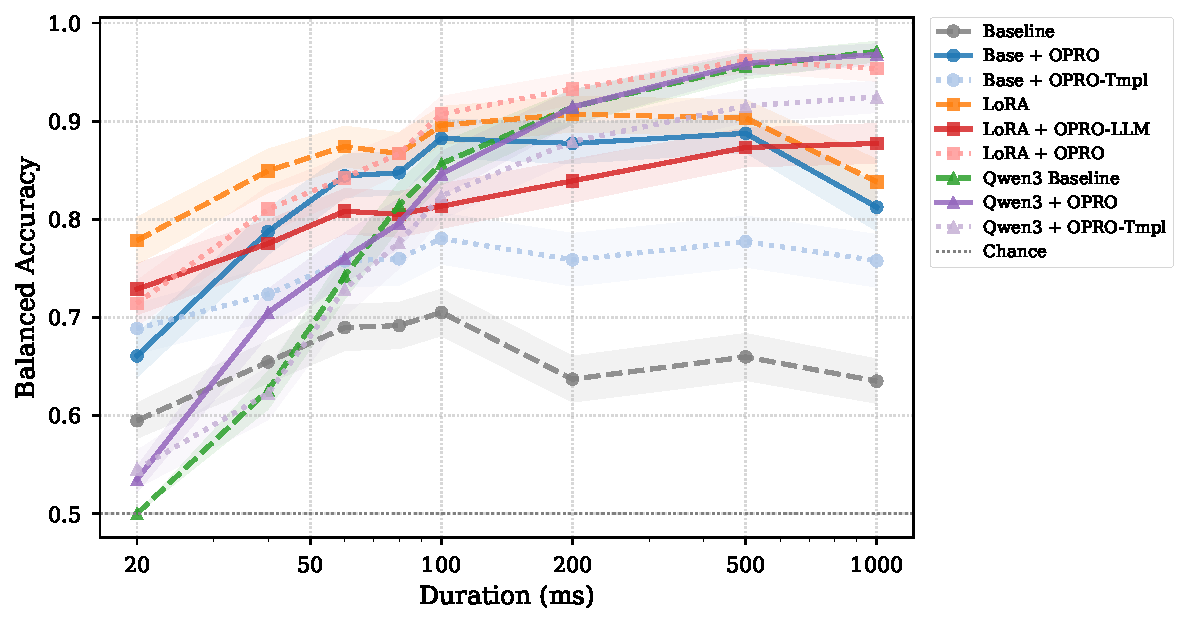
\includegraphics[width=0.95\linewidth]{figures/Fig_Duration.pdf}
\caption{Balanced accuracy versus segment duration (20--1000\,ms). Shaded bands indicate 95\% normal-approximation confidence intervals. Adapted models converge to ceiling performance at longer durations; the baseline remains below all other configurations across the entire sweep.}
\label{fig:duration_ba}
\end{figure}

Table~\ref{tab:psychometric_thresholds} reports the DT90 threshold, the minimum duration at which each configuration reaches 90\% balanced accuracy. The baseline model never crosses the 90\% criterion at any tested duration, but this
reflects a general failure of the zero-shot configuration rather than a temporal resolution
bottleneck specifically: its overall BA of 64.0\% indicates systematic misclassification
even at 1000\,ms. The concept of temporal integration limit is most meaningful for adapted
models that achieve ceiling performance at longer durations and degrade only as duration
decreases. Prompt optimization alone (Base+OPRO-LLM) likewise fails to reach the 90\% criterion within the tested range (DT90 $>$\,1000\,ms), indicating that while OPRO substantially raises overall BA (Section~\ref{subsec:overall_performance}), it cannot push temporal resolution past the 90\% threshold. LoRA fine-tuning reduces DT90 to 329\,ms [87, 1000], and the combination LoRA+OPRO-Tmpl achieves the lowest DT90 at 96\,ms [88, 133]. At this scale, the fine-tuned model integrates speech evidence from segments shorter than a typical syllable nucleus ($\sim$200\,ms), approaching the temporal resolution of human listeners~\cite{kocinski2016time}.

\begin{table}[ht]
\centering
\caption{Psychometric thresholds with 95\% bootstrap confidence intervals. Values are reported as point estimate [CI]. Censored values (\textit{italic with~$\dagger$}) indicate thresholds outside the tested range.}
\label{tab:psychometric_thresholds}
\begin{tabular}{lcccc}
\toprule
\textbf{Configuration} & \textbf{DT50 (ms)} & \textbf{DT75 (ms)} & \textbf{DT90 (ms)} & \textbf{SNR75 (dB)} \\
\midrule
Base+Hand & \textit{$<$20\,$^\dagger$} & \textit{$>$1000\,$^\dagger$} & \textit{$>$1000\,$^\dagger$} & \textit{$>$20\,$^\dagger$} \\
Base+OPRO-LLM & \textit{$<$20\,$^\dagger$} & 34 [31, 672] & \textit{$>$1000\,$^\dagger$} & \textit{$<$$-$10\,$^\dagger$} \\
LoRA+Hand & \textit{$<$20\,$^\dagger$} & \textit{$<$20\,$^\dagger$} & 329 [87, 1000] & \textit{$<$$-$10\,$^\dagger$} \\
LoRA+OPRO-Tmpl & \textit{$<$20\,$^\dagger$} & 27 [22, 32] & 96 [88, 133] & $-$16\textsuperscript{$\star$} \\
\midrule
Qwen3+Hand & 20 [20, 25] & 62 [57, 69] & 175 [146, 222] & $-$13\textsuperscript{$\star$} \\
Qwen3+OPRO-LLM & \textit{$<$20\,$^\dagger$} & 56 [47, 68] & 179 [155, 221] & $-$12\textsuperscript{$\star$} \\
Qwen3+OPRO-Tmpl & \textit{$<$20\,$^\dagger$} & 69 [59, 80] & 371 [211, 757] & \textit{$<$$-$10\,$^\dagger$} \\
\midrule
Silero VAD v5\textsuperscript{$\ddagger$} & \textit{$<$20\,$^\dagger$} & 81 & 196 & $-$7 \\
\bottomrule
\end{tabular}

\vspace{0.4em}
\begin{flushleft}
\footnotesize
$^\dagger$\,\textit{Censored:} the true threshold lies outside the tested range. $<$20\,ms means the criterion is already met at the shortest tested duration; $>$1000\,ms means it is never met. $<$$-$10\,dB and $>$+20\,dB indicate censoring below and above the tested SNR range. Non-censored values (upright) are interpolated within the tested range.\\[0.3em]
$^\star$\,Interpolated from extended SNR evaluation ($-20$ to $+20$\,dB) on the three top-performing configurations. Point estimates only (no bootstrap CI).
\end{flushleft}
\end{table}

The frozen Qwen3-Omni model exhibits high temporal robustness across the tested duration range, maintaining high balanced accuracy at short segments (Figure~\ref{fig:duration_ba}). The frozen Qwen3-Omni model achieves a DT90 of 175\,ms [146, 222] (Table~\ref{tab:psychometric_thresholds}), positioning it between LoRA+Hand (329\,ms) and the fully adapted LoRA+OPRO-Tmpl (96\,ms). Prompt optimization does not measurably improve Qwen3's temporal resolution (DT90 179\,ms [155, 221]).

The nature of detection errors changes qualitatively across the duration axis. At the shortest duration (20\,ms), errors are almost exclusively false negatives (speech clips misclassified as non-speech), with FNR-to-FPR ratios exceeding 24:1 for LoRA+OPRO-Tmpl and 134:1 for Base+Hand.\footnote{At 20\,ms: LoRA+OPRO-Tmpl FNR\,=\,0.480, FPR\,=\,0.020 (ratio 24:1); Base+Hand FNR\,=\,0.938, FPR\,=\,0.007 (ratio 134:1). See Table~\ref{tab:error_counts} for full confusion matrices.} Qwen3-Omni exhibits this asymmetry in its most extreme form: at 20\,ms, it classifies every clip as NONSPEECH (0\% speech recall, 100\% specificity), suggesting that the MoE architecture requires a minimum amount of acoustic evidence before committing to a speech decision. This all-or-nothing behavior contrasts with the gradual degradation observed in dense models and may reflect a hard evidence threshold imposed by the MoE routing mechanism, which only activates speech-relevant experts when sufficient acoustic energy is present. At the longest duration (1000\,ms), the pattern partially reverses for adapted models: LoRA+OPRO-Tmpl achieves near-perfect speech recall (FNR $= 0.004$) but shows increased false alarms (FPR $= 0.089$), indicating a shift from conservative to liberal detection as temporal context increases. Figure~\ref{fig:supp_error_duration} decomposes this evolution, showing FPR and FNR trajectories across the full duration axis for selected configurations.

\begin{figure}[t]
\centering

\includegraphics[width=0.95\linewidth]{figures/Fig_Supp_ErrorByDuration.pdf}
\caption{False-positive rate (FPR, dashed) and false-negative rate (FNR, solid) as a function of segment duration for selected configurations. At short durations, errors are dominated by false negatives (missed speech); as duration increases, adapted models shift toward low FNR with slightly elevated FPR.}
\label{fig:supp_error_duration}
\end{figure}


\subsection{Primary Paired Comparisons and Statistical Significance}
\label{subsec:results_primary_comparisons}

Because all configurations are evaluated on the same degraded clips, we report \emph{paired} effect sizes for a small set of \emph{primary, pre-specified} comparisons. For each comparison (A vs.\ B), we compute $\Delta$BA $=$ BA(A)$-$BA(B), so negative values indicate that system B achieves higher balanced accuracy. We report $\Delta$BA with 95\% confidence intervals (CI) and assess statistical significance using McNemar's exact test on paired outcomes, applying Holm correction across the primary comparisons. Because each base clip generates 22 correlated variants, we additionally report cluster-bootstrap $p$-values ($p_{\mathrm{cluster}}$, $B = 10{,}000$) that resample at the base-clip level to account for within-clip dependence. For comparisons with large effect sizes ($\Delta$BA $>$ 5\,pp), both methods agree; for the smallest effect (Qwen3+Hand vs.\ Qwen3+OPRO-LLM, $\Delta$BA $= 0.3$\,pp), the cluster-aware test fails to reject the null ($p_{\mathrm{cluster}} = 0.093$), indicating that the marginal OPRO gain on Qwen3 is not statistically reliable.

\begin{table}[t]
\centering
\caption{Primary paired comparisons on the evaluation set. $\Delta$BA $=$ BA(A)$-$BA(B).
Discordant counts are from McNemar contingency tables: $n_{01}$ counts clips where A is
correct and B is incorrect; $n_{10}$ counts clips where A is incorrect and B is correct.}
\label{tab:primary_comparisons}
\footnotesize
\setlength{\tabcolsep}{3pt}
\renewcommand{\arraystretch}{1.12}
\resizebox{\linewidth}{!}{%
\begin{tabular}{lccccccc}
\toprule
Comparison (A vs.\ B) & $\Delta$BA & 95\% CI & $p$ (raw) & $p_{\mathrm{Holm}}$ & Disc.\ rate & $n_{01}$ & $n_{10}$ \\
\midrule
Baseline vs Base+OPRO & -0.186 & [-0.199, -0.173] & $<$10$^{-10}$ & $<$10$^{-10}$ & 0.268 & 869 & 4840 \\
Baseline vs LoRA+BasePrompt & -0.224 & [-0.236, -0.212] & $<$10$^{-10}$ & $<$10$^{-10}$ & 0.285 & 650 & 5428 \\
LoRA+BasePrompt vs LoRA+OPRO & -0.069 & [-0.079, -0.059] & $<$10$^{-10}$ & $<$10$^{-10}$ & 0.104 & 379 & 1850 \\
LoRA+OPRO\_Classic vs LoRA+OPRO\_Open & +0.093 & [0.079, 0.106] & $<$10$^{-10}$ & $<$10$^{-10}$ & 0.169 & 2787 & 813 \\
Qwen3 Baseline vs Qwen3+OPRO & -0.003 & [-0.006, 0.000] & 0.014 & 0.014 & 0.029 & 275 & 337 \\
LoRA+OPRO-Tmpl vs Qwen3 Baseline & +0.022 & [0.015, 0.029] & $<$10$^{-10}$ & $<$10$^{-10}$ & 0.074 & 1030 & 559 \\
\bottomrule
\end{tabular}%
}
\end{table}


\subsection{Noise Robustness}
\label{subsec:results_snr}

Figure~\ref{fig:snr_ba} displays balanced accuracy as a function of SNR ($-10$ to $+20$\,dB). The LoRA-adapted configurations are nearly flat across the entire SNR range, maintaining high BA even under heavy additive noise. Specifically, all LoRA-based models achieve SNR75 below $-10$\,dB (Table~\ref{tab:psychometric_thresholds}), the lowest tested level, indicating near-complete invariance to the noise conditions in our evaluation bank. In contrast, the Qwen2-Base model fails to reach the 75\% criterion at any tested SNR (SNR75 $>$ $+20$\,dB).

\begin{figure}[t]
\centering
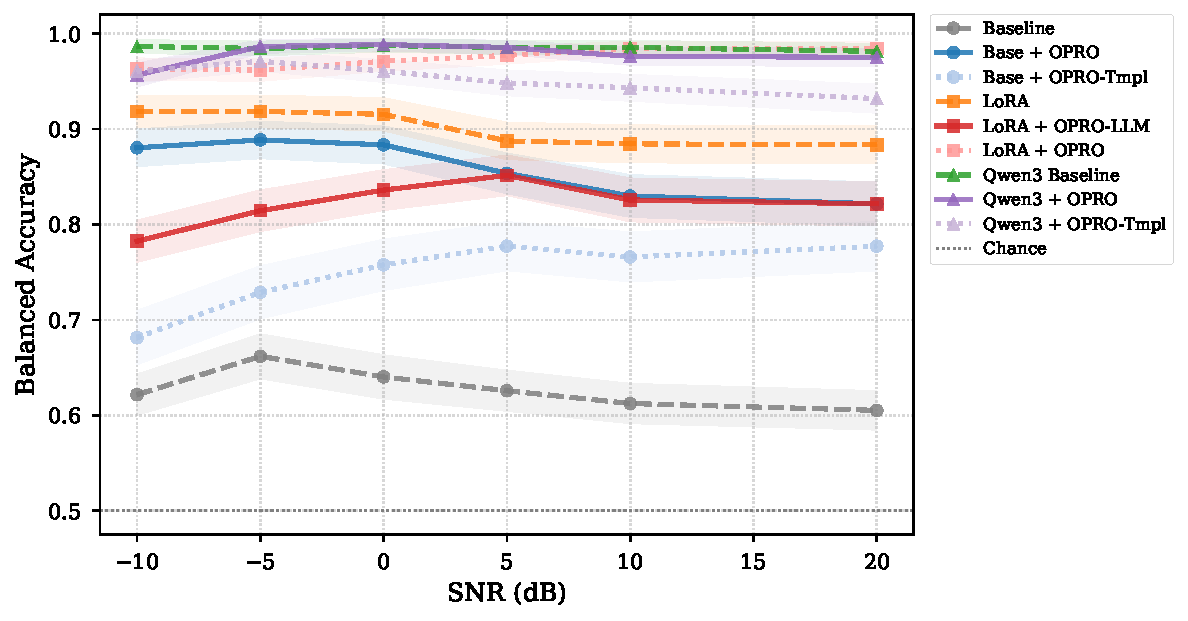
\includegraphics[width=0.95\linewidth]{figures/Fig_SNR.pdf}
\caption{Balanced accuracy versus SNR. The standard range ($-10$ to $+20$\,dB) is shown for all configurations; the three top performers are additionally evaluated at $-15$ and $-20$\,dB (extended range). Shaded bands indicate 95\% normal-approximation confidence intervals.}
\label{fig:snr_ba}
\end{figure}

LoRA fine-tuning contributes the largest share of noise invariance. Base+OPRO-LLM achieves a marked improvement over Base+Hand but remains consistently below LoRA-based performance across all SNR levels, confirming that weight adaptation, not prompting, is the primary driver of robustness to additive noise. The frozen Qwen3-Omni model exhibits high noise robustness without any parameter updates, but its performance at extreme noise conditions is slightly below that of LoRA+OPRO-Tmpl.

To resolve the censored SNR75 values for the three top-performing configurations, we extended the evaluation to $-15$ and $-20$\,dB. The results reveal a sharp performance cliff between $-10$ and $-15$\,dB that differentiates fine-tuned from frozen models. LoRA+OPRO-Tmpl maintains 83.3\% BA at $-15$\,dB and degrades to chance only at $-20$\,dB (51.2\%), yielding an interpolated SNR75 of $-16$\,dB. In contrast, both Qwen3 configurations collapse abruptly: Qwen3+Hand drops from 98.7\% at $-10$\,dB to 51.6\% at $-15$\,dB (SNR75 $\approx -13$\,dB), while Qwen3+OPRO-LLM falls to 50.0\% (SNR75 $\approx -12$\,dB), indicating pure NONSPEECH bias. These results suggest that LoRA fine-tuning provides approximately 3--4\,dB of additional noise resilience beyond what the larger frozen model achieves, and that prompt optimization does not improve noise robustness at extreme SNR levels.


\subsection{Reverberation and Spectral Filtering}
\label{subsec:results_reverb_filter}

Figure~\ref{fig:reverb_ba} shows robustness to reverberation. As shown in Table~\ref{tab:r04_dimension_means}, adapted models are also highly robust to spectral filtering. The baseline shows marked sensitivity to both axes, particularly to highpass filtering, which removes the low-frequency energy that dominates voiced speech. LoRA-adapted models and the frozen Qwen3-Omni configuration remain high and stable across all conditions on both axes, with LoRA+OPRO-Tmpl consistently achieving the smallest performance variability.

\begin{figure}[t]
\centering
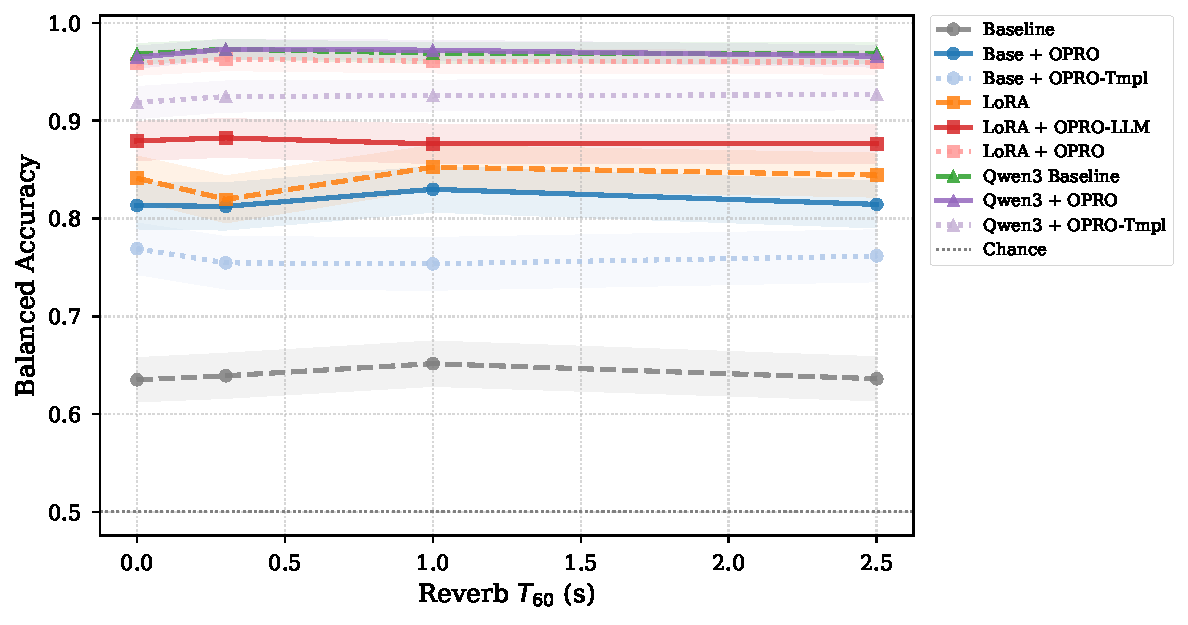
\includegraphics[width=0.95\linewidth]{figures/Fig_Reverb.pdf}
\caption{Balanced accuracy versus reverberation time RT60 (0--2.5\,s). Shaded bands indicate 95\% normal-approximation confidence intervals.}
\label{fig:reverb_ba}
\end{figure}

\begin{table}[t]
\centering
\caption{Mean balanced accuracy (\%) within each degradation axis (macro-average over the conditions in that axis). Bold indicates column-wise best.}
\label{tab:r04_dimension_means}
\footnotesize
\setlength{\tabcolsep}{4pt}
\renewcommand{\arraystretch}{1.12}
\begin{tabular}{llcccc}
\toprule
\textbf{Model} & \textbf{Configuration} & \textbf{Duration} & \textbf{SNR} & \textbf{Reverb} & \textbf{Filter} \\
\midrule
Qwen2-Audio-7B & Base + Hand & 65.9 & 62.8 & 64.0 & 62.1 \\
Qwen2-Audio-7B & Base + OPRO-LLM & 82.5 & 86.0 & 81.8 & 78.7 \\
Qwen2-Audio-7B & Base + OPRO-Tmpl & 75.1 & 74.8 & 76.0 & 74.7 \\
\midrule
Qwen2-Audio-7B & LoRA + Hand & 86.4 & 90.1 & 83.9 & 83.2 \\
Qwen2-Audio-7B & LoRA + OPRO-LLM & 81.5 & 82.2 & 87.9 & 88.0 \\
Qwen2-Audio-7B & LoRA + OPRO-Tmpl & \textbf{87.4} & 97.4 & 96.1 & 96.2 \\
\midrule
Qwen3-Omni-30B & Hand & 79.8 & \textbf{98.5} & \textbf{97.0} & 96.7 \\
Qwen3-Omni-30B & OPRO-LLM & 81.1 & 97.8 & 96.9 & \textbf{96.8} \\
Qwen3-Omni-30B & OPRO-Tmpl & 77.7 & 95.3 & 92.4 & 92.2 \\
\bottomrule
\end{tabular}
\end{table}


\subsection{Prompting Strategies: Generative vs.\ Deterministic}
\label{subsec:results_prompting_strategies}

Our experimental matrix crossed model configurations with two distinct optimization strategies: \textit{OPRO-LLM} (which generates natural-language instructions) and \textit{OPRO-Template} (which selects from fixed, structured formats). The winning prompts for each configuration are reported in Table~\ref{tab:winning_prompts}. Comparing these reveals a sharp divergence in preference depending on whether the model has undergone parameter adaptation.

\textbf{Frozen models prefer natural language.}
For both Qwen2-Base and Qwen3-Omni, the generative OPRO-LLM strategy outperforms the deterministic OPRO-Template. On Qwen2-Base, OPRO-LLM reaches 82.6\% BA compared to 75.1\% for the Template approach. Similarly, Qwen3-Omni achieves its peak (91.4\%) with OPRO-LLM, whereas the Template approach drops to 87.8\%. The divergence extends beyond overall accuracy: Qwen3-Omni's DT90 under OPRO-LLM is 179\,ms, but degrades to 371\,ms under OPRO-Template (Table~\ref{tab:psychometric_thresholds}), indicating that the structured template format also impairs the frozen model's temporal resolution. Per-duration analysis reveals the mechanism: at 200\,ms, OPRO-Template shifts the operating point toward higher speech recall (97.5\% vs.\ 95.5\% for the baseline) at the expense of nonspeech recall (78.4\% vs.\ 87.4\%). This $\sim$9\,pp specificity collapse pulls balanced accuracy below the 90\% threshold at durations where the baseline prompt is comfortably above it. The structured definitions in the template appear to bias the frozen model toward liberal detection, a trade-off that the baseline's simpler instruction avoids. This suggests that general-purpose instruction-tuned models benefit from the linguistic nuances and flexible phrasing that the meta-LLM can generate.

\textbf{Fine-tuned models prefer rigid structure.}
In contrast, the LoRA-adapted model shows the opposite behavior. It achieves its best performance (93.3\%) with OPRO-Template, which enforces a strict definitions-based structure. Notably, applying the generative OPRO-LLM to the LoRA model actually \emph{degrades} performance to 84.0\%, worse than the unoptimized LoRA baseline (86.4\%). This gap is statistically confirmed: OPRO-Template outperforms OPRO-LLM on the LoRA model by 9.3\,pp (Table~\ref{tab:primary_comparisons}, $p < 10^{-10}$). In fact, applying OPRO-LLM to the LoRA model not only reduces overall BA but also collapses temporal resolution (DT90 $>$\,1000\,ms versus 329\,ms for the unoptimized LoRA), confirming that misaligned prompts can destroy capabilities established through fine-tuning.

This reversal indicates that LoRA fine-tuning, which used a strict A/B training format (Section~\ref{subsubsec:lora_method}), specializes the model to respond to structured, low-perplexity prompts. The success of OPRO-Template on the LoRA model likely stems from its structured definitions format, which aligns with the deterministic training distribution, even though evaluation uses open-ended generation for all cells. Consequently, natural-language variations generated by OPRO-LLM drift away from the narrow distribution the model was fine-tuned on, introducing output variability that degrades classification accuracy. We defer the mechanistic interpretation of this reversal to Section~\ref{subsec:disc_opro_saturation}, where we analyze it in terms of prompt--adaptation alignment. We conclude that while input-space optimization is universally beneficial, the \textit{type} of prompt must align with the model's training history: natural language for frozen models, and structured templates for fine-tuned ones.

\textbf{Template stability across seeds.}
The OPRO-Template search uses a mini-dev budget of $N = 20$ samples per iteration with a fixed random seed, raising the question of whether the winning template is stable across different search runs. Table~\ref{tab:multiseed_opro} reports full-test-set BA for five random seeds per model. LoRA and Qwen3 configurations show moderate stability ($\sigma = 2.4$ and $1.1$\,pp, respectively), with the reported seed (42) yielding the best or tied-best result for LoRA (3 of 5 seeds converge to the same template) and a representative result for Qwen3. The Base model exhibits higher variance ($\sigma = 6.1$\,pp) driven by a single outlier seed (789) that selects a qualitatively different template.

\begin{table}[t]
\centering
\caption{Multi-seed OPRO-Template stability. $\text{BA}_{\text{clip}}$ (\%) on the full test set for five random seeds. The reported results use seed~42 (bold).}
\label{tab:multiseed_opro}
\footnotesize
\setlength{\tabcolsep}{4pt}
\renewcommand{\arraystretch}{1.12}
\begin{tabular}{lccccc|cc}
\toprule
\textbf{Model} & \textbf{s42} & \textbf{s123} & \textbf{s456} & \textbf{s789} & \textbf{s1024} & \textbf{Mean} & \textbf{Std} \\
\midrule
Base   & \textbf{75.1} & 75.1 & 75.1 & 61.4 & 75.1 & 72.3 & 6.1 \\
LoRA   & \textbf{93.3} & 91.5 & 87.7 & 93.3 & 93.3 & 91.8 & 2.4 \\
Qwen3  & \textbf{87.8} & 86.3 & 87.8 & 89.5 & 87.8 & 87.9 & 1.1 \\
\bottomrule
\end{tabular}
\end{table}


\subsection{Error Analysis}
\label{subsec:results_error_analysis}

To interpret the balanced-accuracy gains in terms of operational errors, we decompose each configuration's predictions into false-positive rate (FPR; false alarms on NONSPEECH) and false-negative rate (FNR; missed SPEECH). Figure~\ref{fig:recall_tradeoff} visualizes the resulting trade-off as a sensitivity--specificity scatter plot, where the upper-right corner represents simultaneously high SPEECH recall and high NONSPEECH recall.

\begin{table*}[t]
\centering
\caption{Error profile (confusion matrix counts and derived error rates) for each configuration, aggregated over the full test set (10{,}670 SPEECH and 10{,}670 NONSPEECH samples).}
\label{tab:error_counts}
\footnotesize
\setlength{\tabcolsep}{4pt}
\renewcommand{\arraystretch}{1.12}
\begin{tabular}{llcccccc}
\toprule
\textbf{Model} & \textbf{Config} & \textbf{TP} & \textbf{TN} & \textbf{FP} & \textbf{FN} & \textbf{FPR} & \textbf{FNR} \\
\midrule
Qwen2-Audio-7B & Base + Hand      &  3{,}423 & 10{,}236 &    434 & 7{,}247 & 0.041 & 0.679 \\
Qwen2-Audio-7B & Base + OPRO-LLM  &  7{,}966 &  9{,}664 & 1{,}006 & 2{,}704 & 0.094 & 0.253 \\
Qwen2-Audio-7B & Base + OPRO-Tmpl &  7{,}655 &  8{,}368 & 2{,}302 & 3{,}015 & 0.216 & 0.283 \\
\midrule
Qwen2-Audio-7B & LoRA + Hand      &  8{,}797 &  9{,}640 & 1{,}030 & 1{,}873 & 0.097 & 0.176 \\
Qwen2-Audio-7B & LoRA + OPRO-LLM  & 10{,}135 &  7{,}799 & 2{,}871 &    535 & 0.269 & 0.050 \\
Qwen2-Audio-7B & LoRA + OPRO-Tmpl &  9{,}904 & 10{,}004 &    666 &    766 & 0.062 & 0.072 \\
\midrule
Qwen3-Omni-30B & Hand      &  9{,}328 & 10{,}109 &    561 & 1{,}342 & 0.053 & 0.126 \\
Qwen3-Omni-30B & OPRO-LLM  &  9{,}518 &  9{,}981 &    689 & 1{,}152 & 0.065 & 0.108 \\
Qwen3-Omni-30B & OPRO-Tmpl &  9{,}626 &  9{,}111 & 1{,}559 & 1{,}044 & 0.146 & 0.098 \\
\bottomrule
\end{tabular}
\end{table*}

\begin{figure}[t]
\centering
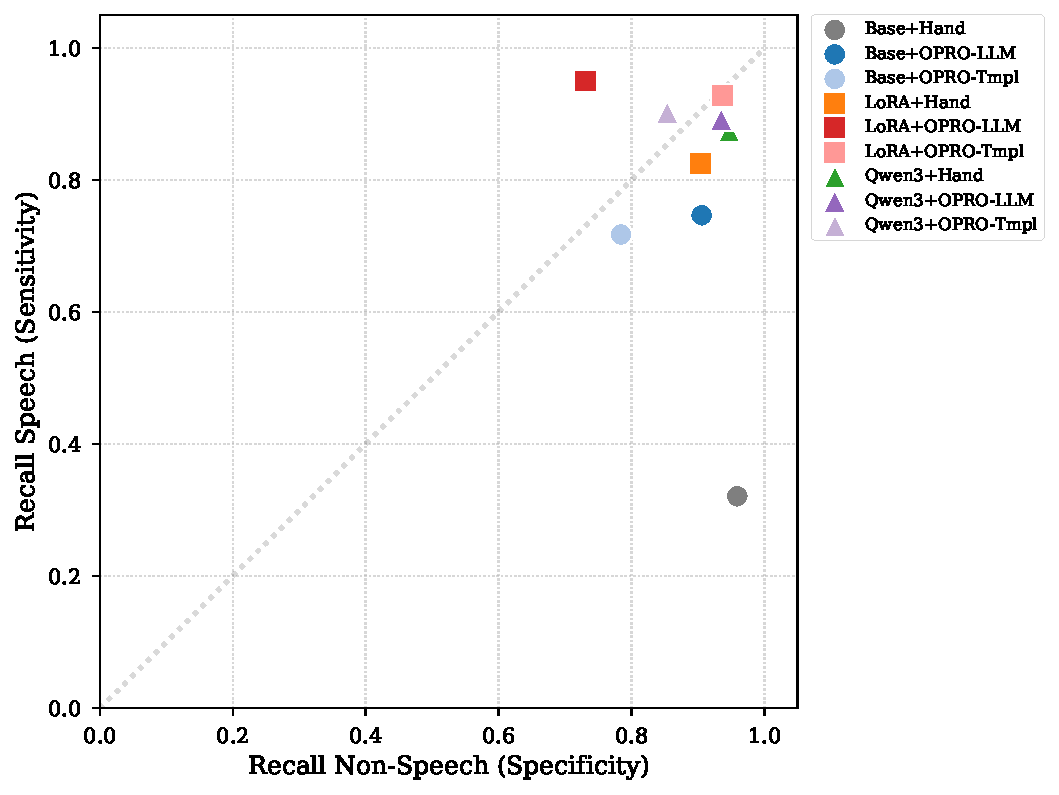
\includegraphics[width=0.85\linewidth]{figures/Fig_Tradeoff.pdf}
\caption{Recall trade-off by configuration. Each point shows (NONSPEECH recall, SPEECH recall) aggregated over the full evaluation set. Ideal operating point: upper-right corner.}
\label{fig:recall_tradeoff}
\end{figure}

Three distinct operating regimes emerge. First, the \emph{conservative baseline}: Qwen2-Base achieves very high specificity (low FPR) at the cost of extremely low sensitivity, effectively defaulting to NONSPEECH under uncertainty. Second, the \emph{sensitivity-recovered} regime: OPRO shifts the operating point sharply toward higher SPEECH recall, recovering the model's ability to detect speech under degradation, but introducing more false alarms. Third, the \emph{balanced} regime: LoRA fine-tuning raises both sensitivity and specificity simultaneously, and the addition of OPRO-Tmpl on top of LoRA further refines specificity while maintaining near-ceiling SPEECH recall. LoRA+OPRO-Tmpl occupies the position closest to the ideal upper-right corner, confirming it as the best-balanced configuration in the matrix.

The frozen Qwen3-Omni model enters the balanced regime without parameter updates, achieving high recall on both classes. However, its error profile is less favorable than LoRA+OPRO-Tmpl: its SPEECH recall is slightly lower and its NONSPEECH recall does not reach the fine-tuned model's level, consistent with the 2.2\,pp gap observed in overall BA (Table~\ref{tab:overall_performance}).


\subsection{Non-Speech Category Difficulty}
\label{subsec:results_nonspeech_categories}

The preceding error analysis aggregates across all NONSPEECH categories. We now decompose performance by ESC-50 category to identify which acoustic classes drive the residual false positives.

The inclusion of all 50 ESC-50 categories in the NONSPEECH class creates a natural difficulty gradient. Categories containing vocalizations, which share acoustic features with speech such as harmonic structure, temporal modulation, and voiced energy, are substantially harder to classify correctly. Across the 17~categories with human or animal vocalizations (3{,}740 test samples), the best model (LoRA+OPRO-Tmpl) achieves 87.1\% NONSPEECH accuracy, compared to 98.2\% on the remaining 33~environmentally unambiguous categories, an 11.1~percentage-point gap. Three categories prove particularly challenging: \emph{laughing} (31.8\% accuracy), \emph{coughing} (56.6\%), and \emph{crying baby} (77.3\%). The frozen Qwen3-Omni model exhibits a different difficulty profile: \emph{coughing} is substantially easier (90.9\%), suggesting that its broader pretraining distribution better separates impulsive respiratory sounds from speech. These error rates reveal the acoustic boundary at which LALMs conflate vocalization with speech, a boundary that any VAD system must negotiate.

Figure~\ref{fig:esc50_heatmap} provides the complete per-category accuracy breakdown across all nine configurations, revealing that the difficulty gradient is not uniform across adaptation strategies. Environmental sounds (e.g., rain, wind, engine) are correctly classified at near-ceiling rates by all adapted models, while human vocalizations (laughing, coughing, snoring) form a persistent confusion cluster that even the best configuration fails to fully resolve.

\begin{figure}[t]
\centering
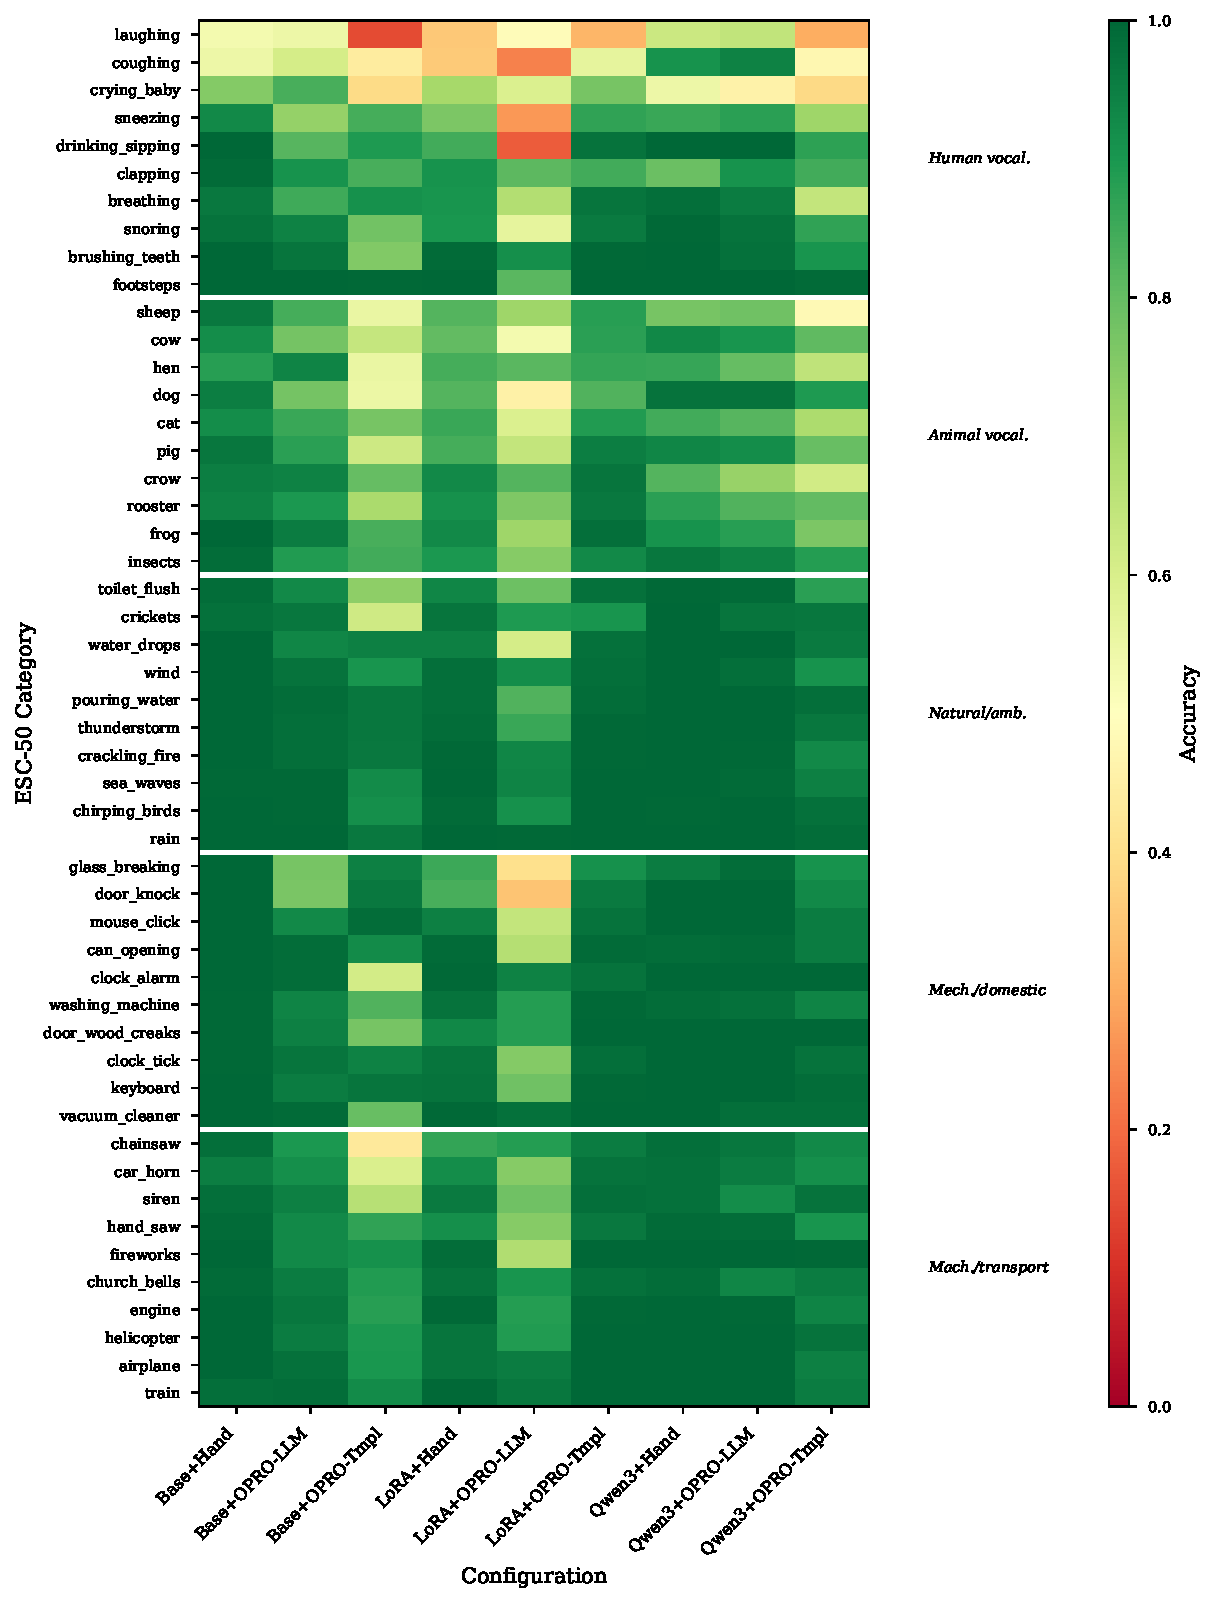
\includegraphics[width=0.95\linewidth]{figures/esc50_heatmap.pdf}
\caption{NONSPEECH accuracy per ESC-50 category across all nine configurations, grouped by acoustic type. Warmer colors indicate lower accuracy (more false positives). Human and animal vocalizations form a consistent difficulty cluster.}
\label{fig:esc50_heatmap}
\end{figure}


\subsection{Summary of Findings}
\label{subsec:results_summary}

The results across all nine cells and 22 degradation conditions converge on a consistent picture:
targeted parameter adaptation on a smaller dense model achieves the highest robustness,
surpassing both prompt-only optimization and a frozen MoE model with 4.4$\times$ more parameters.
The following section examines the mechanistic reasons for this hierarchy and its practical
implications.


%%%%%%%%%%%%%%%%%%%%%%%%%%%%%%%%%%%%%%%%%%%%%%%%%%%%%%%%%%%%%%%%%%%%%%%%%%%%%%%
\section{Discussion}
\label{sec:discussion}
%%%%%%%%%%%%%%%%%%%%%%%%%%%%%%%%%%%%%%%%%%%%%%%%%%%%%%%%%%%%%%%%%%%%%%%%%%%%%%%

The preceding results indicate that, under our experimental conditions, targeted adaptation outperforms architectural scaling, but leave open the question of \emph{where} the performance bottleneck resides and \emph{why} different adaptation strategies interact as they do. We now address these mechanistic questions.

\subsection{Where Does the Temporal Bottleneck Reside?}
\label{subsec:disc_temporal}

The audio encoder in Qwen2-Audio is a Whisper-large-v3 encoder that operates on 25\,ms frames with 10\,ms hop size, producing feature representations at a temporal granularity well below our shortest test duration of 20\,ms. If the encoder itself can resolve sub-frame events, then the DT90 of the zero-shot baseline ($>$1000\,ms) cannot be attributed to an encoder-side resolution limit. Instead, the bottleneck lies downstream: the language model must map a sequence of acoustic embeddings to a categorical decision, and this mapping, learned during general-purpose pretraining, is not calibrated for fine-grained temporal evidence under degradation.

LoRA adaptation operates precisely at this interface. By inserting low-rank updates into the attention projections of the language model, LoRA likely refines how acoustic features are aggregated across the temporal dimension and aligned to the decision vocabulary. The reduction from DT90 $>$ 1000\,ms (Base+Hand) to 96\,ms (LoRA+OPRO-Tmpl) suggests that the pretrained model discards or underweights short-duration acoustic evidence, and that a modest number of trainable parameters suffices to recover this information. Prompt optimization alone does not reduce DT90 below the tested range ($>$\,1000\,ms), indicating that instruction rephrasing cannot compensate for a misaligned feature--decision mapping at the temporal level, despite substantially improving overall balanced accuracy.

This interpretation aligns with prior work on LALM temporal limitations. Wang et al.~\cite{wang2025timeaudio} traced temporal imprecision to projection layers that downsample the encoder's output, while Sridhar et al.~\cite{sridhar-etal-2025-enhancing} found that standard pretraining does not instill fine-grained temporal reasoning. Our results extend these observations to the detection setting: even binary clip-level decisions, far simpler than temporal grounding or onset localization, require explicit adaptation to exploit short-duration cues reliably.

The frozen Qwen3-Omni model maintains high balanced accuracy at short durations (Figure~\ref{fig:duration_ba}) without any parameter updates. One plausible explanation is that its MoE routing mechanism, trained on a broader distribution of audio tasks and modalities, has already learned to retain short-duration acoustic features in a subset of its expert pathways. However, without the ability to fine-tune these pathways for the specific decision boundary, the frozen model cannot push temporal resolution to its minimum.

Verifying this hypothesis would require probing intermediate representations before and
after LoRA adaptation. For instance, training linear classifiers on encoder outputs versus
post-attention representations for short-duration clips would determine whether temporal
evidence is present but underweighted in the frozen model (supporting our interpretation)
or genuinely absent at that processing stage.

\subsection{Scaling versus Adaptation: A Cost--Benefit Analysis}
\label{subsec:disc_cost_benefit}

The adaptation hierarchy (Section~\ref{subsec:results_summary}) reveals a practical tension between two deployment philosophies. The frozen Qwen3-Omni model offers high out-of-the-box robustness (91.1\% BA) with zero training cost, but at substantially higher inference cost: 30.5B total parameters, A100-class GPUs, and no quantization. The LoRA-adapted Qwen2-Audio achieves higher accuracy (93.3\% BA) on consumer-grade hardware (RTX 3090, 4-bit quantization), but requires a curated training set and a fine-tuning pipeline. Although we do not report measured per-sample latency (Section~\ref{subsec:limitations}), the 4-bit quantized 7B model is expected to offer substantially higher throughput per dollar compared to the unquantized 30B model, given the $4.4\times$ parameter ratio and the absence of quantization in Qwen3-Omni. The total wall-clock time for the Qwen2-Audio matrix run (LoRA training + OPRO optimization + evaluation of all six Qwen2 cells) was approximately 13.4~hours on a single NVIDIA A100-SXM4-80GB GPU. The OPRO-LLM optimization alone requires ${\sim}$15{,}000--18{,}000 forward passes through the target model (Section~\ref{subsubsec:opro_llm}), while OPRO-Template requires only ${\sim}$2{,}400 (Section~\ref{subsubsec:opro_template}), an order-of-magnitude asymmetry that favors the template approach when computational budget is limited.

This trade-off maps to two distinct deployment scenarios. For \emph{rapid prototyping and general-purpose deployment}, the frozen MoE model with OPRO is attractive: no labeled data are needed, adaptation consists of prompt search over a small development set, and the resulting system generalizes across degradation axes. For \emph{robustness-sensitive or resource-constrained systems} (such as embedded VAD in hearing aids, acoustic monitoring in noisy industrial environments, or forensic speech detection), the LoRA path is preferable. The 2.2\,pp accuracy advantage and the near-complete noise invariance (SNR75 $< -10$\,dB) may be operationally decisive when false negatives carry high cost, and the smaller model footprint enables deployment on edge hardware. We note, however, that the LoRA model was trained exclusively on clean audio (Section~\ref{subsec:limitations}); the observed robustness to noise and reverberation emerges from generalization rather than explicit exposure to degraded conditions.

The complementarity of OPRO and LoRA further informs this analysis. OPRO-LLM provides the largest marginal gain on the frozen base model (+18.6\,pp), but the best OPRO variant on the already-adapted LoRA model (OPRO-Tmpl, +6.9\,pp) shows diminishing returns. This diminishing return suggests that prompt optimization and weight adaptation partly address the same failure modes (conservative decision thresholds and sensitivity to degradation) through different mechanisms. When both are available, their benefits compound but do not simply add, consistent with the hypothesis that OPRO reshapes the input to the decision layer while LoRA reshapes the decision layer itself.

\subsection{OPRO Dynamics: Why Gains Saturate on Strong Models}
\label{subsec:disc_opro_saturation}

The near-zero OPRO gain on Qwen3-Omni (+0.3\,pp) contrasts with the large gains on Qwen2-Base (+18.6\,pp). This asymmetry has implications for the broader applicability of prompt optimization. On a model that already handles degradation robustly, the prompt's role is reduced to formatting and instruction clarity; there is little latent capability for the prompt to unlock. Conversely, on a model with strong latent representations but a poorly calibrated decision strategy, prompt optimization may act as a lightweight recalibration: we hypothesize that it shifts the decision boundary and redirects the model's attention toward diagnostic acoustic features, yielding large gains without modifying a single weight. Verifying this hypothesis would require attention-map or probing analyses, which we leave for future work.

This observation suggests a diagnostic use for OPRO: the magnitude of prompt-optimization gain serves as a proxy for how much of a model's failure is attributable to instruction misalignment versus representational limitations. Large OPRO gains indicate ``unlockable'' capability; small gains indicate that the bottleneck lies deeper, in the model's internal representations, and that weight adaptation or architectural changes are needed.

We note that the magnitude of OPRO gain is measured relative to the shared baseline prompt;
a prompt that happens to be better suited to one architecture than another would shift the
apparent gain independently of true latent capability. Controlled experiments with multiple
baseline prompts would be needed to disentangle prompt-architecture affinity from recoverable
capability, and we leave this investigation for future work.

The interaction between OPRO variant and adaptation state further refines this diagnostic. OPRO-LLM degrades LoRA performance (84.0\% vs.\ 86.4\% unoptimized; Section~\ref{subsec:results_prompting_strategies}), while OPRO-Template yields the best result (93.3\%). This reversal is consistent with the interpretation that LoRA fine-tuning narrows the model's effective input distribution: the A/B training format (Section~\ref{subsubsec:lora_method}) conditions the model to expect structured, low-perplexity prompts, and the natural-language variations generated by OPRO-LLM fall outside this distribution.

Examining the winning prompts clarifies the mechanism. The OPRO-LLM prompt generated for LoRA (``\textit{Classify this audio as SPEECH or NON-SPEECH, focusing on short and noisy clips}'') uses a concise free-form format that diverges from the structured A/B format used during LoRA training. In contrast, the winning OPRO-Template (``\textit{Detect human speech. Treat the following as NONSPEECH: pure tones/beeps, clicks\ldots}'') provides structured category definitions that closely mirror the deterministic training distribution, even though both prompts trigger the same open-ended decoding path at evaluation time. The practical implication is that prompt optimization strategy must be matched to the model's training history: generative search for frozen models, constrained template search for fine-tuned ones.

\paragraph{Confidence calibration.}
%Beyond classification accuracy, adaptation also affects how well a model's confidence aligns with its true performance. Figure~\ref{fig:supp_calibration} presents a reliability diagram comparing the first-token probability ($p_{\text{first\_token}}$) against empirical accuracy. The LoRA-adapted model (ECE $= 0.062$) is well-calibrated: its confidence scores closely track the diagonal, and its predictions concentrate in the 0.9--1.0 range, indicating decisive and accurate classification. In contrast, the frozen Base + OPRO-LLM model (ECE $= 0.456$) exhibits systematic overconfidence: it assigns moderate confidence ($\sim$0.3--0.5) to predictions that achieve $\sim$0.87 accuracy, suggesting that the model's internal representations support better performance than its confidence reflects. This miscalibration gap further supports the interpretation that LoRA recalibrates not only the feature--decision mapping (Section~\ref{subsec:disc_temporal}) but also the model's uncertainty quantification, an important property for deployment scenarios where prediction confidence informs downstream decisions.
Beyond classification accuracy, adaptation also affects how well a model's confidence aligns with its true performance. Figure~\ref{fig:supp_calibration} presents a reliability diagram comparing the first-token probability ($p_{\text{first\_token}}$) against empirical accuracy for the two Qwen2-Audio configurations where token-level probabilities are available.\footnote{Qwen3-Omni is excluded because its inference pipeline does not expose per-token probabilities through the same interface; extending this analysis to MoE architectures requires model-specific instrumentation.} The LoRA-adapted model (ECE $= 0.062$) is well-calibrated: its confidence scores closely track the diagonal, and its predictions concentrate in the 0.9--1.0 range, indicating decisive and accurate classification. In contrast, the frozen Base + OPRO-LLM model (ECE $= 0.456$) exhibits systematic overconfidence: it assigns moderate confidence ($\sim$0.3--0.5) to predictions that achieve $\sim$0.87 accuracy, suggesting that the model's internal representations support better performance than its confidence reflects. This miscalibration gap further supports the interpretation that LoRA recalibrates not only the feature--decision mapping (Section~\ref{subsec:disc_temporal}) but also the model's uncertainty quantification, an important property for deployment scenarios where prediction confidence informs downstream decisions.


\begin{figure}[t]
\centering

\includegraphics[width=0.95\linewidth]{figures/Fig_Supp_Calibration.pdf}
%\caption{Reliability diagram comparing first-token probability ($p_{\text{first\_token}}$) against empirical accuracy. Top: calibration curves with ECE (Expected Calibration Error); shaded areas show miscalibration gap relative to the diagonal. Bottom: distribution of predictions across confidence bins. The LoRA-adapted model is well-calibrated (ECE $= 0.062$), while the base model shows systematic overconfidence (ECE $= 0.456$).}
\caption{Reliability diagram comparing first-token probability ($p_{\text{first\_token}}$) against empirical accuracy for Qwen2-Audio configurations. Top: calibration curves with Expected Calibration Error (ECE); shaded areas indicate miscalibration relative to the diagonal. Bottom: distribution of predictions across confidence bins. LoRA adaptation yields well-calibrated confidence (ECE $= 0.062$), whereas the base model with prompt optimization shows systematic overconfidence (ECE $= 0.456$).}
\label{fig:supp_calibration}
\end{figure}

\subsection{Limitations}
\label{subsec:limitations}

Several limitations bound the generalizability of our findings. First, all speech material is drawn from VoxConverse, an English-language conversational corpus. The extent to which the adaptation hierarchy and psychometric thresholds transfer to other languages, speaking styles (e.g., read speech, whispered speech), or non-Western acoustic environments remains untested.

Second, our evaluation is restricted to binary clip-level detection (SPEECH vs.\ NONSPEECH). We do not evaluate temporal localization (onset/offset timestamps), speaker diarization, or multi-class sound event detection. While the psychometric framework is class-agnostic by design and could be extended to other target events, the specific adaptation gains reported here may not transfer to tasks requiring finer-grained temporal or semantic resolution.

Third, our psychometric protocol varies each degradation axis independently while holding others
at neutral values. This one-factor-at-a-time design enables clear attribution of performance
changes to individual acoustic factors, following standard psychoacoustic methodology, but
does not capture interactions between degradation axes. In realistic deployment scenarios,
degradations co-occur (e.g., short segments in noisy, reverberant environments), and the
adaptation hierarchy established here may shift under combined stress. Extending the
evaluation to factorial or representative combinations of degradation conditions is a natural
direction for future work.

Fourth, the NONSPEECH class is drawn exclusively from ESC-50, which comprises isolated
environmental sounds rather than the continuous background signals (sustained music,
multi-talker babble, ambient noise) encountered in typical VAD deployment. Similarly, the
Silero-based quality filter (speech ratio $\geq 0.8$) retains only clips with high speech
occupancy, excluding the onset/offset boundary regions that constitute the most challenging
cases for practical VAD. These design choices prioritize controlled evaluation and label
integrity at the cost of ecological representativeness. Extending the evaluation to
continuous-background corpora and to boundary-case speech clips would test whether the
adaptation hierarchy generalizes beyond the clean-segment regime.

Fifth, Qwen3-Omni is evaluated only as a frozen model (see Section~\ref{subsubsec:qwen3_config}
for details on the architectural constraints that preclude PEFT).
The frozen evaluation thus establishes a lower bound on what the MoE architecture can achieve;
a complete comparison would require fine-tuning both models under equivalent conditions.

Sixth, the training set for LoRA (3{,}072 clips) consists exclusively of clean, undegraded audio. The observed noise and reverberation robustness emerges entirely from generalization, not from exposure to degraded training examples. Whether augmenting the training set with degraded samples would further improve robustness, or whether it would introduce overfitting to specific degradation profiles, is an open question.

Seventh, Qwen2-Audio uses 4-bit NF4 quantization while Qwen3-Omni runs unquantized. This asymmetry places the smaller model at a representational disadvantage; however, as noted in Section~\ref{subsec:overall_performance}, the fact that the adapted 7B model still outperforms the unquantized 30B model reinforces our conclusion regarding the efficacy of parameter adaptation over architectural scaling.

Eighth, the OPRO-Template search uses a fixed random seed (seed~42) with a mini-dev budget of $N = 20$ samples per iteration, yielding a score resolution of 0.05. A multi-seed validation (Table~\ref{tab:multiseed_opro}) confirms moderate stability for LoRA ($\sigma = 2.4$\,pp across 5 seeds) and Qwen3 ($\sigma = 1.1$\,pp), though the Base model exhibits higher variance ($\sigma = 6.1$\,pp). The reported seed yields the best or tied-best result for LoRA (3 of 5 seeds converge to the same template), which should be considered when interpreting the absolute performance values.

Ninth, we do not report per-sample inference latency. The cost-benefit analysis in Section~\ref{subsec:disc_cost_benefit} is based on architectural parameters (model size, quantization, GPU class) rather than measured throughput. Direct latency benchmarking under controlled conditions would strengthen the deployment recommendations.

% TODO: REVIEW - verify karan24_interspeech (pyannote) removed from refs.bib if not cited elsewhere
Additionally, while we include Silero VAD~\cite{silero_vad_github} as a reference point in Table~\ref{tab:overall_performance}, this comparison is indicative rather than comprehensive. Silero is designed for continuous-stream processing, and our clip-level evaluation protocol does not leverage its temporal context modeling. A rigorous comparison against dedicated lightweight VAD systems would require an experimental design accounting for differences in output format, temporal granularity, and deployment constraints.


%%%%%%%%%%%%%%%%%%%%%%%%%%%%%%%%%%%%%%%%%%%%%%%%%%%%%%%%%%%%%%%%%%%%%%%%%%%%%%%
\section{Conclusion}
\label{sec:conclusion}
%%%%%%%%%%%%%%%%%%%%%%%%%%%%%%%%%%%%%%%%%%%%%%%%%%%%%%%%%%%%%%%%%%%%%%%%%%%%%%%

We presented a psychometric evaluation framework for assessing Large Audio-Language Models as low-level acoustic detectors under controlled degradation. By sweeping 22 conditions across four axes (segment duration, signal-to-noise ratio, reverberation, and spectral filtering), we constructed robustness curves that expose where and how each adaptation strategy fails, going beyond the aggregate metrics reported in standard benchmarks.

Our central finding is that, under the conditions tested, targeted parameter adaptation on a smaller model outperforms architectural scaling without adaptation. A 7B dense model fine-tuned with LoRA and optimized with OPRO-Tmpl achieves 93.3\% balanced accuracy and a task-specific temporal integration limit of 96\,ms [88, 133], surpassing a frozen 30B Mixture-of-Experts model (Qwen3+Hand, 91.1\%) that requires substantially greater compute. This result holds across all four degradation axes and is statistically confirmed via paired McNemar tests with Holm--Bonferroni correction ($p < 10^{-10}$; Table~\ref{tab:primary_comparisons}).

Four practical recommendations follow from these results. First, for robustness-sensitive applications where missed detections carry high cost (acoustic monitoring, forensic analysis, hearing device preprocessing), LoRA fine-tuning on curated data is the preferred path: it yields the highest robustness to noise (SNR75 $< -10$\,dB) and the finest temporal resolution (DT90 $\approx$ 96\,ms) at low inference cost. Second, for rapid prototyping or scenarios where labeled training data are unavailable, frozen MoE models with OPRO offer a strong baseline that requires only a small development set for prompt search. Third, the magnitude of OPRO gain on a given model serves as a diagnostic signal: large gains indicate recoverable capability through instruction tuning, while small gains suggest that the performance bottleneck lies in the model's internal representations. Fourth, prompt optimization strategy must be matched to the model's training history: frozen models benefit from generative natural-language optimization (OPRO-LLM), while fine-tuned models require deterministic templates (OPRO-Template) to maintain alignment with their training distribution.

The psychometric framework itself constitutes an independent contribution. By treating detection accuracy as a function of stimulus parameters, analogous to human psychometric functions, we derive compact thresholds (DT90, SNR75) that summarize robustness in interpretable units. These thresholds are directly transferable to other sound events by relabelling the positive class, offering a general methodology for probing LALM behavior under acoustic stress.

Future work should extend this evaluation along three directions. First, multilingual and multi-style speech corpora would test whether adaptation gains are language-dependent. Second, temporal localization tasks (onset/offset detection, diarization) would reveal whether the temporal integration limits identified here impose fundamental constraints on finer-grained analyses. Third, LoRA adaptation of MoE architectures would disentangle the contributions of expert routing and weight specialization to acoustic robustness.

\bibliographystyle{plainnat}
\bibliography{refs}

\end{document}